%%%%%%%%%%%%%%%%%%%%%%%%%%%%%%%%%%%%%%%%%%%%%%%%
%% Compile the master file!
%% 		Slides: Antonio Machicao y Priemer
%% 		Course: GK Linguistik
%%%%%%%%%%%%%%%%%%%%%%%%%%%%%%%%%%%%%%%%%%%%%%%%


%%%%%%%%%%%%%%%%%%%%%%%%%%%%%%%%%%%%%%%%%%%%%%%%%%%%
%%%             Metadata                         
%%%%%%%%%%%%%%%%%%%%%%%%%%%%%%%%%%%%%%%%%%%%%%%%%%%%      

\title{Grundkurs Linguistik}

\subtitle{Semantik I}

\author[aMyP]{
	{\small Antonio Machicao y Priemer}
	\\
	{\footnotesize \url{http://www.linguistik.hu-berlin.de/staff/amyp}}
%	\\
%	\href{mailto:mapriema@hu-berlin.de}{mapriema@hu-berlin.de}}
}

\institute{Institut für deutsche Sprache und Linguistik}

\date{ }

%\publishers{\textbf{6. linguistischer Methodenworkshop \\ Humboldt-Universität zu Berlin}}

%\hyphenation{nobreak}


%%%%%%%%%%%%%%%%%%%%%%%%%%%%%%%%%%%%%%%%%%%%%%%%%%%%
%%%             Preamble's End                   
%%%%%%%%%%%%%%%%%%%%%%%%%%%%%%%%%%%%%%%%%%%%%%%%%%%%      


%%%%%%%%%%%%%%%%%%%%%%%%%      
\huberlintitlepage[22pt]

\iftoggle{toc}{
\frame{
\begin{multicols}{2}
	\frametitle{Inhaltsverzeichnis}\tableofcontents
	%[pausesections]
\end{multicols}
}
}


%%%%%%%%%%%%%%%%%%%%%%%%%%%%%%%%%%
%%%%%%%%%%%%%%%%%%%%%%%%%%%%%%%%%%
%%%%%LITERATURE:

%% Allgemein
\nocite{Glueck&Roedel16a}
\nocite{Luedeling2009a}
\nocite{Meibauer&Co07a} 
\nocite{Repp&Co15a} 

%% Morphologie
%\nocite{Eisenberg04}

%% Syntax
%\nocite{Adger04a}
%\nocite{Altmann&Hofmann08a} % Satztypen & Satzmodi
%\nocite{Altmann93a} % Satztypen & Satzmodi
%\nocite{Brandt&Co06a} 
%\nocite{Fanselow&Sascha87a}
%\nocite{Fanselow&Sascha93a}
%\nocite{Fries&MyP16b} % Akzeptabilität
%\nocite{Fries16a} % Grammatikalität
%\nocite{Fries&MyP16d} % Kompetenz vs Performanz
%\nocite{Fries&MyP16c} % GG
%\nocite{Fries&MyP16a} % X-Bar-Theorie
%\nocite{Fries16e} % Satztyp
%\nocite{Fries16d} % Satzmodus 
\nocite{Grewendorf&Co91a} 
%\nocite{MyP17b} % Kerngrammatik
%\nocite{MyP18a} % Konstituententest
\nocite{MyP18b} % Kopf
%\nocite{MyP18c} % Phrase
%\nocite{MyP18s} % Funktionale Kategorie
\nocite{MyP18t} % Argumentstruktur
%\nocite{MuellerS13f} 
%\nocite{MuellerS15b}
%\nocite{Stechow&Sternefeld88a}
%\nocite{Sternefeld06a}
%\nocite{Sternefeld06b}
%\nocite{Woellstein10a} % Topologisches Feldermodell

%% Semantik & Pragmatik
\nocite{Loebner15a} %% Semantics
\nocite{Loebner15b} %% Semantics
\nocite{Lohnstein11} %% Semantics
\nocite{MyP16a} %% Bikonditional
\nocite{Partee&Co93a} %% Semantics
\nocite{ZimmermannT&Sternefeld13a} %% Semantics


%%%%%%%%%%%%%%%%%%%%%%%%%%%%%%%%%%
%%%%%%%%%%%%%%%%%%%%%%%%%%%%%%%%%%
\begin{frame}
\frametitle{Begleitlektüre}

\begin{itemize}
	\item AM S.~95--106
	\item \citet{Lohnstein11}: Kapitel 4 (S.~34--49)
\end{itemize}
\end{frame}


%%%%%%%%%%%%%%%%%%%%%%%%%%%%%%%%%%%
\section{Semantik}
%%%%%%%%%%%%%%%%%%%%%%%%%%%%%%%%%%%
%
\subsection{Einführung}

\iftoggle{sectoc}{
	\frame{
		%\begin{multicols}{2}
		\frametitle{~}
		\tableofcontents[currentsubsection,subsubsectionstyle=hide]
		%\end{multicols}
	}
}
%%%%%%%%%%%%%%%%%%%%%%%%%%%%%%%%%%%

\begin{frame}
\frametitle{Einführung}

\begin{itemize}
	\item Semantik: Bedeutungslehre
	\item []
	\item Teildisziplin der \textbf{Linguistik} 
	\item[]
	\item Aufgabe: Erfassen der \textbf{Bedeutung} von einfachen und zusammengesetzten \textbf{natürlichsprachlichen Ausdrücken} 

\end{itemize}

\end{frame}


%%%%%%%%%%%%%%%%%%%%%%%%%%%%%%%%%%%%%%%%
\begin{frame}
	\frametitle{Einführung}

\begin{itemize}
	\item Durch morphologische und syntaktische Kompetenz \ras Produktion von unendlich vielen Wörtern und Sätzen
	\item[]
	\item Aufgabe der Semantik: 
	
	\begin{itemize}
		\item Welche Kenntnisse besitzen wir, um diese unendlich vielen sprachlichen (einfachen oder komplexen) Ausdrücke zu \textbf{verstehen} (oder zu \textbf{produzieren})?
		
		\item Wie muss unsere \textbf{semantische Kompetenz} aussehen? (Welche Restriktionen besitzt sie?)
		
		\item Welche sind die \textbf{zugrunde liegenden Fähigkeiten}?
	\end{itemize}

\end{itemize}

\end{frame}
	
	
%%%%%%%%%%%%%%%%%%%%%%%%%%%%%%%%%%%%%%%%
\begin{frame}
\frametitle{Einführung}

\begin{itemize}
	\item Gegenstandsbereiche anderer Teilbereiche der Linguistik sind \gqq{leichter} zu erfassen
		
		\begin{itemize}
			\item Phonologie, die Morphologie und die Syntax \ras Datensammlungen (Korpora oder in Tonaufnahmen)
		\end{itemize}
	
	\item []	
	\item Bedeutung lässt sich schwer messen oder erfassen
		
		\begin{itemize}
			\item Methoden: muttersprachliche Intuition, psycholinguistische Experimente
		\end{itemize}
		
	\item[]	
	\item Semantik als Teildisziplin der \textbf{Semiotik}:
	
	\begin{itemize}
		\item Semiotik: Lehre der Zeichen
		
		\item \textbf{Semantik}: Disziplin, die sich mit der Bedeutung von \textbf{Zeichen im Allgemeinen} (vgl.\ Symbol, Ikone, Index) und mit der \textbf{Beziehung} zwischen der Form und der \textbf{Bedeutung} eines Zeichens befasst
	\end{itemize} 
	
\end{itemize}

\end{frame}


%%%%%%%%%%%%%%%%%%%%%%%%%%%%%%%%%%%%%
%
\subsection{Zeichen}
%
\iftoggle{sectoc}{
	\frame{
		%\begin{multicols}{2}
		\frametitle{~}
		\tableofcontents[currentsubsection,subsubsectionstyle=hide]
		%\end{multicols}
	}
}
%%%%%%%%%%%%%%%%%%%%%%%%%%%%%%%%%%%%%%%%

\begin{frame} \frametitle{Zeichen}

\begin{columns}
	
\begin{column}{.5\textwidth}

\begin{itemize}
	\item Zeichen bestehen aus zwei Komponenten:
	
	\begin{itemize}
		\item \textbf{Inhaltsseite}
		\item \textbf{Ausdrucksseite}
	\end{itemize}
	
	\item[]
	
	\item Untersuchung der Beziehung zwischen Inhalts- und Ausdrucksseite u.\,a. durch Ferdinand de Saussure und Karl Bühler (Organonmodell) zu Beginn des XX. Jhs.
	
\end{itemize}

\end{column}
%%
%%
\begin{column}{.5\textwidth}

\begin{figure}
	\begin{center}
		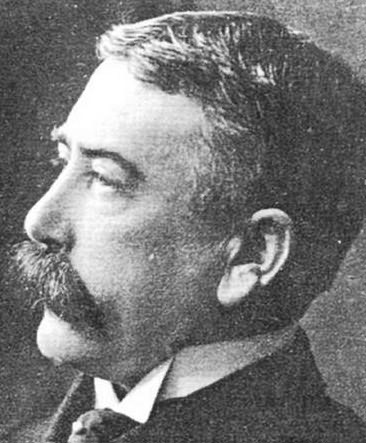
\includegraphics[scale=.3]{material/Ferdinand_de_Saussure}	
	\end{center}
	
	\caption{Ferdinand de Saussure}	
\end{figure}
	
\end{column}

\end{columns}

\end{frame}


%%%%%%%%%%%%%%%%%%%%%%%%%%%%%%%%%%%%%%%%
\begin{frame} \frametitle{Zeichen}

\begin{itemize}
	\item \citet{Saussure16x}: Ein linguistisches Zeichen ist nicht eine Verbindung zwischen einem Ding und einem Namen, sondern zwischen einem \textbf{Konzept} (frz.\ signifié/""dt.\ Signifikat) und einem \textbf{Lautmuster} (frz.\ signifiant/""dt.\ Signifikant).
\end{itemize}	

%\begin{center}
%	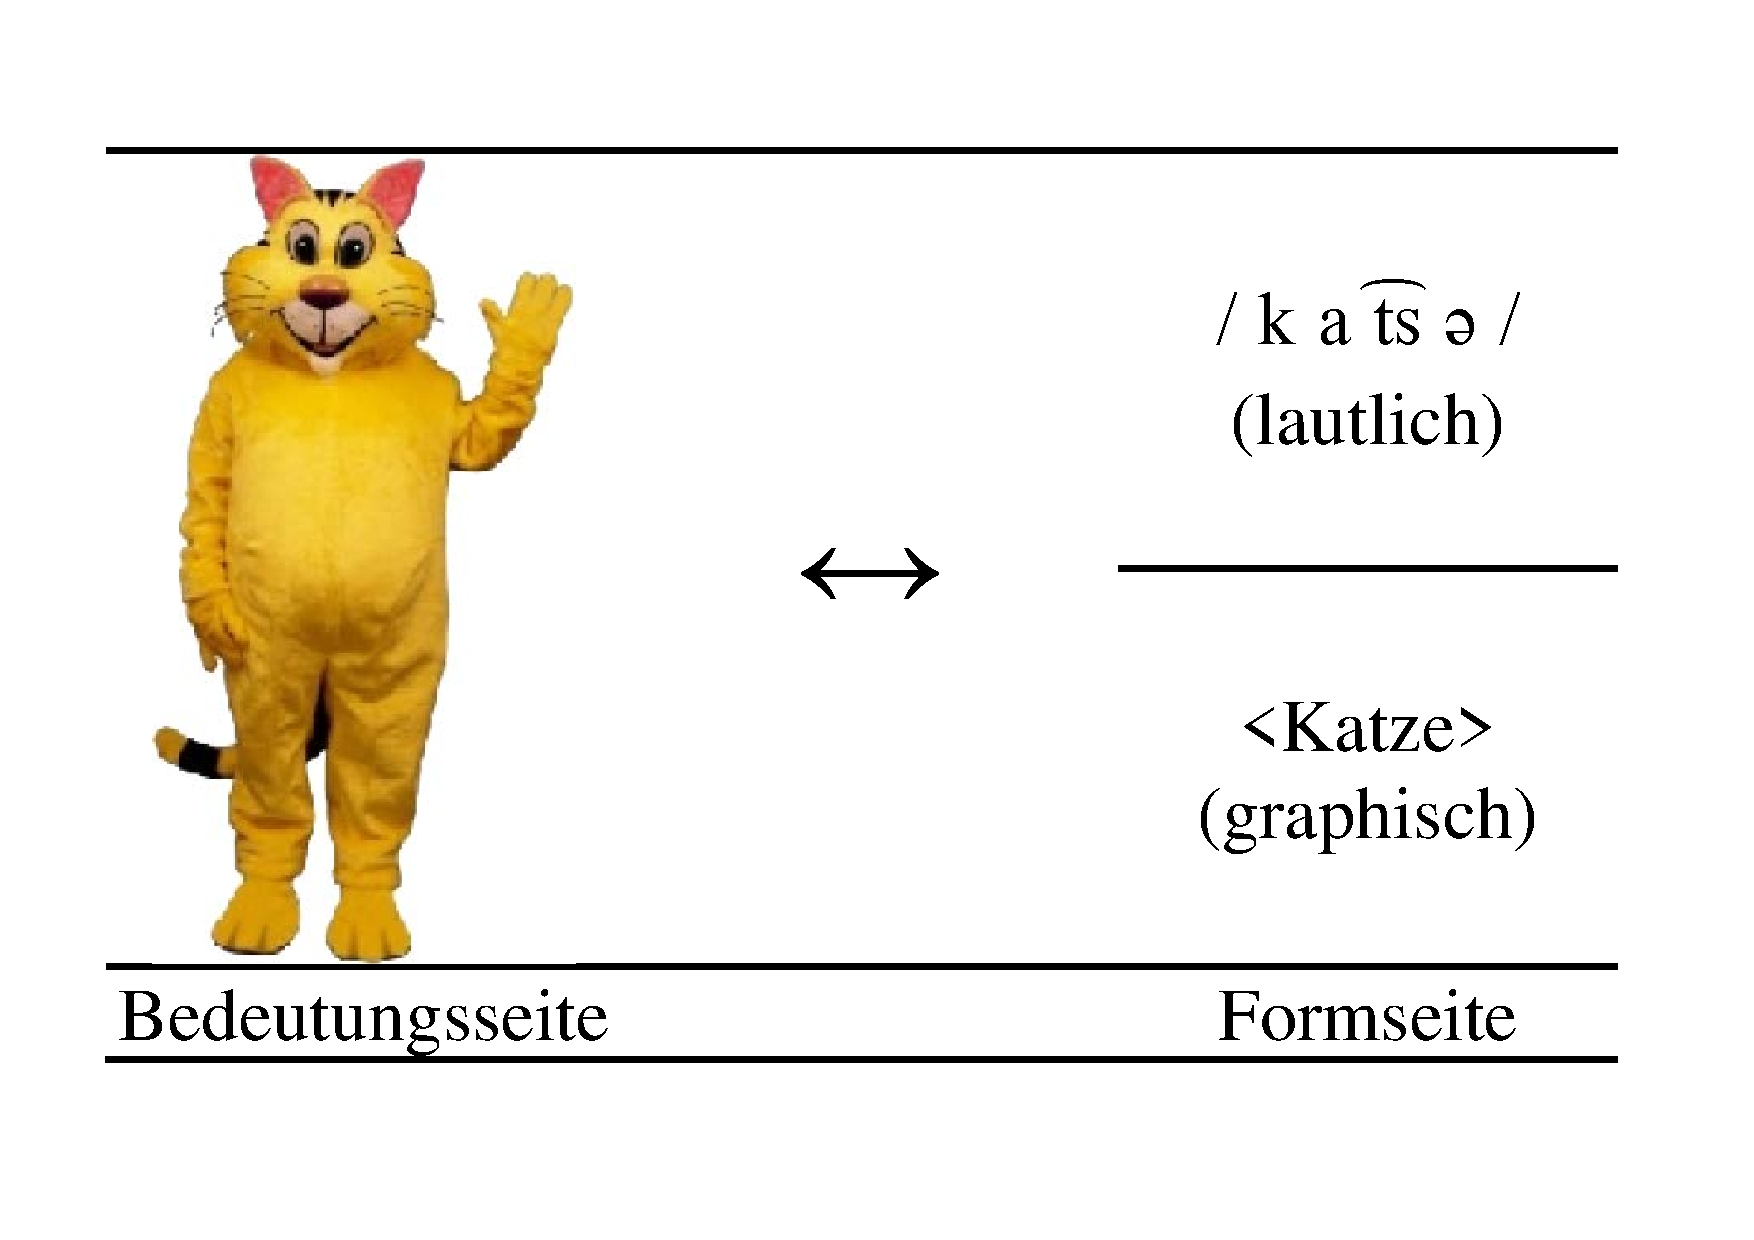
\includegraphics[scale=.2]{material/01SSZeichenKatze}	
%\end{center}

\begin{figure}
	\centering
\scalebox{.75}{\begin{tikzpicture}
\draw[black] (-1,0)--(6,0);
\draw[black](-1,0.5)--(6,0.5);
\draw[black](-1,4.5)--(6,4.5);
\draw[black](4,2.5)--(6,2.5);
\node at (1,2.5){
\includegraphics[scale=0.12]{material/gelbe-katze2}};
\node[align=center] at (5,3.5){/\textipa{ka\t{ts}@}/ \\ (lautlich)};
\node[align=center] at (5,1.5){\abe{Katze} \\ (graphisch)};
\node[above] at (1,-0.1){Bedeutungsseite};
\node[above] at (5,0){Formseite};
\node at (3,2.5){{\huge $\leftrightarrow$}};
\end{tikzpicture}}
\caption{Zeichenmodell nach Saussure (1916/1967)}
\end{figure}

\end{frame}	


%%%%%%%%%%%%%%%%%%%%%%%%%%%%%%%%%%%%%%%%
\begin{frame} \frametitle{Zeichen}

\begin{itemize}
	\item \textbf{Bilaterale Zeichenkonzeption} von de Saussure wurde ergänzt: Mit sprachlichen Zeichen beziehen wir uns \textbf{nicht auf Begriffe}, sondern \textbf{auf Referenten} in der Welt, auf \gqq{Gegenstände}.
\end{itemize}

	\begin{figure}
	\centering
	\small
	\scalebox{.74}{\begin{tikzpicture}
		\draw[dashed] (-4,0)--(4,0);
		\draw[black] (4,0)--(0,3)--(-4,0);
		\node[above, align=center] at (-4.5,0){/\textipa{ka\t{ts}@}/ \\ \abe{Katze}}; 
		\node[below, align=center] at (-4.5,0){\textbf{AUSDRUCK} \\Signifiant (Saussure), Zeichen (Peirce), \\ Symbol (Odgen/Richards)};
		\node[below] at (0,0){\emph{steht für}};
		\node[left] at (-1.9,1.8){\emph{geknüpft an}};
		\node[right] at (1.9,1.8){\emph{bezieht sich auf}};
		\node[above, align=center] at (0,3){\textbf{BEGRIFF} \\ Signifié (Saussure), Sinn (Frege), Interpretant (Peirce),\\ Intension (Carnap), Idee, Gedanke \ldots \\ {[KATZE]}};
		\node[above] at (4.8,0){
\includegraphics[scale=0.04]{material/gelbe-katze2}};
		\node[below, align=center] at (4.5,0){ \textbf{REFERENT}\\ Gegenstand (Frege, Peirce) \\ Extension (Carnap), Denotation (Russell)};
		\end{tikzpicture}}
	\caption{Das Semiotische Dreieck nach Odgen/""Richards (1923)}
\end{figure}


	
\end{frame}	


%%%%%%%%%%%%%%%%%%%%%%%%%%%%%%%%%

\begin{frame}
\frametitle{Zeichen}

\begin{itemize}
	\item Ein sprachlicher Ausdruck (Formseite des Zeichens) hat \textbf{keinen direkten Bezug} auf einen Referenten.
	
	\item []	
	
	\item Der Bezug zwischen dem Ausdruck und dem Referenten erfolgt \textbf{durch den Begriff} (in der aktuellen sprachlichen Welt).
	
	\item[]
	
	\item Ein \textbf{Ausdruck} ist an einen \textbf{Begriff} (oder Konzept) gekoppelt, der schließlich die \textbf{Referenz} ermöglicht.
		
\end{itemize}
	
\end{frame}


%%%%%%%%%%%%%%%%%%%%%%%%%%%%%%%%%%%
\begin{frame}
\frametitle{Zeichen}

\begin{itemize}
	\item Wichtige Eigenschaften von Zeichen \citep[vgl.][]{Saussure16x}:
	
	\item[]
		
	\item \textbf{Arbitrarität:} Die Verbindung zwischen Zeichenform und Zeicheninhalt ist willkürlich.
	
	\begin{itemize}
		\item Derselbe Inhalt wird in unterschiedlichen Sprachen durch verschiedene (lautliche) Formen realisiert.
		
		\ea \gq{Katze}: Dt.: Katze, Sp.: gato, Frz.: chat
		\z 
		
		\item Von der Form eines sprachlichen Zeichens kann man nicht auf seinen Inhalt/Referenten schließen (Ausnahme: onomatopoetische Ausdrücke).
	\end{itemize}
	

	
\end{itemize}

\end{frame}


%%%%%%%%%%%%%%%%%%%%%%%%%%%%%%%%%%%
\begin{frame}
	\frametitle{Zeichen}

\begin{itemize}
	\item Wichtige Eigenschaften von Zeichen \citep[vgl.][]{Saussure16x}:

	\item[]
	
	\item \textbf{Konventionalität:} Die Verbindung zwischen Zeichenform und Zeicheninhalt muss in einer Sprachgemeinschaft \textbf{festgelegt} sein, d.\,h. welche Form mit welchem Inhalt verknüpft ist. Dies muss so \textbf{gelernt} werden und kann \textbf{nicht beliebig verändert} werden.
\end{itemize}

\end{frame}

%%%%%%%%%%%%%%%%%%%%%%%%%%%%%%%

\begin{frame}
\frametitle{Zeichen}

\begin{itemize}
	\item Bsp. Gebärdensprachen:
	
	\begin{itemize}
		\item \textbf{Konventionalität} als grundlegendere Eigenschaft
		\item[]
		\item Viele verwendete Zeichen in Gebärdensprachen haben ikonische oder semi-ikonische Eigenschaften.\\
\ras Verbindung zwischen einer Gebärde (Form) und ihrem Inhalt ist nicht immer völlig arbiträr!
		\item[]		
		\item Eine Gebärde kann aber nicht einfach durch eine andere ersetzt werden. \\ \ras \textbf{Konventionalität}
		\item[]
		\item Der ikonische (oder semi-ikonische) Charakter von Gebärden geht mit der Zeit auch verloren, und somit werden diese Zeichen auch \textbf{arbiträr}.
	\end{itemize}
	
\end{itemize}

\end{frame}


%%%%%%%%%%%%%%%%%%%%%%%%%%%%%%%%%%%
%
\subsection{Bedeutung}
%
\iftoggle{sectoc}{
	\frame{
		%\begin{multicols}{2}
		\frametitle{~}
		\tableofcontents[currentsubsection,subsubsectionstyle=hide]
		%\end{multicols}
	}
}
%%%%%%%%%%%%%%%%%%%%%%%%%%%%%%%%%%%%%%

\begin{frame}
\frametitle{Bedeutung}

\begin{itemize}
	\item Bedeutungsbegriff \ras vielschichtig
	\item[]
	\item Bedeutung ist Untersuchungsgegenstand der
	
	\begin{itemize}
		\item Semantik\\ \&
		\item Pragmatik\\ 
		\hfill \dots\  keine klare Trennung!
	\end{itemize}

\pause 
	
	\item Semantik: Untersuchung der kontext\textbf{unabhängigen} Bedeutungsaspekte natürlichsprachlicher Ausdrücke
	\item[]
	\item Pragmatik: Untersuchung der kontext\textbf{abhängigen} Bedeutungsaspekte  natürlichsprachlicher Ausdrücke
\end{itemize}

\end{frame}


%%%%%%%%%%%%%%%%%%%%%%%%%%%%%%%%%%%
\begin{frame}
\frametitle{Bedeutung}

\begin{itemize}
	\item Drei Ebenen der Bedeutung:
	
	\begin{itemize}
		\item Ausdrucksbedeutung (auch Wort-/Satzbedeutung)
		\item Äußerungsbedeutung
		\item Sprecherbedeutung (Kommunikativer Sinn)
	\end{itemize}
	
\end{itemize}

\end{frame}


%%%%%%%%%%%%%%%%%%%%%%%%%%%%%%%%%%%
%
\subsubsection{Ausdrucksbedeutung}
%
%\iftoggle{sectoc}{
%	\frame{
%		%\begin{multicols}{2}
%		\frametitle{~}
%		\tableofcontents[currentsubsection,subsubsectionstyle=hide]
%		%\end{multicols}
%	}
%}
%%%%%%%%%%%%%%%%%%%%%%%%%%%%%%%%%%%%%%%

\begin{frame}
	\frametitle{Ausdrucksbedeutung}


	\begin{itemize}
		\item \textbf{wörtliche Bedeutung}, die sich systematisch aus der Bedeutung der Elemente und der Art der Verknüpfung ableiten lässt
		\item[]
		\item unabhängig vom Äußerungskontext
	\end{itemize} 

\pause 

	\ea \label{ex1}Peter hat das ganze Brot aufgegessen.
	\z

\begin{itemize}
	\item Der Satz in (\ref{ex1}) hat demnach in etwa die Satzbedeutung:\\
	Es gibt ein Individuum, das \textbf{Peter} genannt wird,
	und für dieses Individuum trifft die Eigenschaft zu (\textbf{Deklarativsatz}),
	\textbf{das Brot gänzlich} aufgegessen zu haben (\textbf{Vergangenheitsform}).
\end{itemize}

\end{frame}


%%%%%%%%%%%%%%%%%%%%%%%%%%%%%%%%%%%
%
\subsubsection{Äußerungsbedeutung}
%
%\frame{
%\begin{multicols}{2}
%\frametitle{~}
%	\tableofcontents[currentsection]
%\end{multicols}
%}
%%%%%%%%%%%%%%%%%%%%%%%%%%%%%%%%%%%%%%%

\begin{frame}
\frametitle{Äußerungsbedeutung}

\begin{itemize}
	\item Sie bezieht sich (im Vgl.\ zur Ausdrucksbedeutung) auf die \textbf{in einem bestimmten, situativen Kontext} weiter spezifizierte Bedeutung eines Ausdrucks.

\pause 
	
	\ea \label{ex1b}Peter hat das ganze Brot aufgegessen.
	\z

	\item In (\ref{ex1b}): Wenn Peter an seinem 20.\ Geburtstag am 20.\ Oktober 2010 um 10 Uhr morgens das Brot aufgegessen hat, ist die Äußerung des Satzes um 11 Uhr morgens desselben Tages immer noch wahr.
	\item[]
	\item In diesem Fall redet man auch vom \textbf{Äußerungskontext}, der notwendig ist, um den Satz zu \textbf{disambiguieren} und seine Referenz zu bestimmen (vgl. auch deiktische Ausdrücke).
	
\end{itemize}

\end{frame}


%%%%%%%%%%%%%%%%%%%%%%%%%%%%%%%%%%%
%
\subsubsection{Sprecherbedeutung}
%
%\frame{
%\begin{multicols}{2}
%\frametitle{~}
%	\tableofcontents[currentsection]
%\end{multicols}
%}
%%%%%%%%%%%%%%%%%%%%%%%%%%%%%%%%%%%%%%%

\begin{frame}
\frametitle{Sprecherbedeutung}

\begin{itemize}
	\item Sie meint hingegen die Sprecherintention.
	\item[]
	\item Was meint der Sprecher eigentlich mit der Äußerung des Satzes?

	\ea \label{ex1b}Peter hat das ganze Brot aufgegessen.
	\z

\pause 

	\begin{itemize}
		\item jemanden auffordern, Brot für das Frühstück zu kaufen, weil Peter alles aufgegessen hat
	\end{itemize}
	
	\item In einigen Äußerungskontexten kann die Satzbedeutung eines Ausdrucks stark von seiner Sprecherbedeutung abweichen.
\end{itemize}

\end{frame}


%%%%%%%%%%%%%%%%%%%%%%%%%%%%%%%%%%%

\begin{frame}
\frametitle{Sprecherbedeutung}


	\ea \label{ex2} Da ist die Tür!
	\z
	
	\ea \label{ex3}Das hast du aber toll gemacht!
	\z

\pause 
	
	\begin{itemize}
		\item (\ref{ex2}): Aufforderung, den Raum zu verlassen
		\item[]
		\item (\ref{ex3}): ironischer Kommentar zu jemandem, der etwas falsch gemacht hat
		
	\end{itemize}
	
\end{frame}


%%%%%%%%%%%%%%%%%%%%%%%%%%%%%%%%%%%
%
\subsubsection{Bedeutung: Semantik vs.\ Pragmatik}
%
%\frame{
%\begin{multicols}{2}
%\frametitle{~}
%	\tableofcontents[currentsection]
%\end{multicols}
%}
%%%%%%%%%%%%%%%%%%%%%%%%%%%%%%%%%%%%%%%

\begin{frame}
\frametitle{Bedeutung: Semantik vs.\ Pragmatik}

\begin{itemize}
	\item Ausdrucksbedeutung \ras Gegenstand der Semantik
	\item[]
	\item Sprecherbedeutung \ras Gegenstand der Pragmatik
	\item[]
	\item Äußerungsbedeutung \ras  sowohl in der Semantik (deiktische Elemente, Pronomina) als auch in der Pragmatik (Kontext, Ironie) berücksichtigt
\end{itemize}

\end{frame}


%%%%%%%%%%%%%%%%%%%%%%%%%%%%%%%%%%%
%
\subsection{Lexikalische Semantik}
%
\iftoggle{sectoc}{
	\frame{
		%\begin{multicols}{2}
		\frametitle{~}
		\tableofcontents[currentsubsection,subsubsectionstyle=hide]
		%\end{multicols}
	}
}
%%%%%%%%%%%%%%%%%%%%%%%%%%%%%%%%%%%%%%%

\begin{frame}
\frametitle{Lexikalische Semantik (Wortbedeutung)}

\begin{itemize}
	\item Wortbedeutung \ras \textbf{konventionalisierter} und \textbf{kontextunabhängiger} Inhalt eines Ausdrucks
	\item[]
	\item Lexikalische Semantik:
	
	\begin{itemize}
		\item Erfassung des invariablen Inhalts eines Wortes
		\item Repräsentation und Organisation des Inhalts
		\item Relation zwischen den Bedeutungen verschiedener Ausdrücke
	\end{itemize}
	
	\item[]
	\item Siehe: Merkmalshypothese, Prototypentheorie, Wortfeldrelationen, etc.
\end{itemize}

\end{frame}


%%%%%%%%%%%%%%%%%%%%%%%%%%%%%%%%%%%
%
\subsubsection{Sinnrelationen}
%
%\frame{
%\begin{multicols}{2}
%\frametitle{~}
%	\tableofcontents[currentsection]
%\end{multicols}
%}
%%%%%%%%%%%%%%%%%%%%%%%%%%%%%%%%%%%%%%%

\begin{frame}
\frametitle{Sinnrelationen}

\begin{itemize}
	\item Zusammenhang zwischen den Bedeutungen von Ausdrücken
	\item[]
	\item systematisch erfassbare Relationen:
	
\vspace{5mm}
	
	\begin{itemize}
		\item Synonymie
		\item[]
		\item Hyponymie/""Hyperonymie (Kohyponymie)
		\item[]		
		\item Meronymie
		\item[]
 		\item Antonymie
	\end{itemize}
	
\end{itemize}

\end{frame}


%%%%%%%%%%%%%%%%%%%%%%%%%%%%%%%%%%%

\begin{frame}
%\frametitle{Sinnrelationen}

\begin{block}{Synonymie}
Zwei Ausdrücke $X$ und $Y$ sind Synonyme, wenn der Austausch von $X$ durch $Y$ und umgekehrt in allen Kontexten bei Wahrung der Wahrheit (\emph{salva veritate}) erfolgt.
\end{block}

\begin{itemize}
	\item $X$ ist ein $Y$ und $Y$ ist ein $X$
	\item Bikonditional: $\leftrightarrow$
	
	\eal
		\ex Apfelsine $\leftrightarrow$ Orange
		\ex anfangen $\leftrightarrow$ beginnen
		\ex sterben $\leftrightarrow$ abkratzen
		\ex Treppe $\leftrightarrow$ Stiege
		\ex Brötchen $\leftrightarrow$ Schrippe $\leftrightarrow$ Semmel
	\zl
	
	\item Konnotative, regionale und registerabhängige Unterschiede
\end{itemize}

\end{frame}


%%%%%%%%%%%%%%%%%%%%%%%%%%%%%%%%%%%

\begin{frame}
%\frametitle{Sinnrelationen}

\begin{block}{Hyperonymie/""Hyponymie}
Ein Ausdruck $X$ ist ein Hyperonym von $Y$, wenn die Bedeutung von $Y$ in der Bedeutung von $X$ enthalten ist. Ein Ausdruck $Y$ ist ein Hyponym von $X$, wenn die Bedeutung von $Y$ in der Bedeutung von X enthalten ist.
\end{block}

\begin{itemize}
	\item $Y$ ist ein $X$ (aber $X$ ist nicht notwendigerweise ein $Y$)		
	\item transitive Relation
%	\item[]
	\item Implikation: \ras
	
	\eal 
		\ex Küchenstuhl \ras Stuhl \ras Sitzgelegenheit
		\ex erschie\ss{}en \ras töten
	\zl
		
\end{itemize}

\end{frame}


%%%%%%%%%%%%%%%%%%%%%%%%%%%%%%%%%%%
\begin{frame}
%\frametitle{Sinnrelationen}

\begin{block}{Kohyponymie}
Ein Ausdruck $X$ ist ein Kohyponym von $Z$ (und umgekehrt), wenn die Bedeutung von $X$ und $Z$ in der Bedeutung von $Y$ enthalten ist. Kohyponyme schließen einander aus (Inkompatibilität).
\end{block}

\eal
\ex Drehstuhl/Küchenstuhl \ras Stuhl \ras Sitzgelegenheit
\ex erschießen/erwürgen/erdrosseln \ras töten
\zl

\begin{itemize}
	\item Hyperonymie/Hyponymie: Basis für Taxonomien
\end{itemize}

\end{frame}


%%%%%%%%%%%%%%%%%%%%%%%%%%%%%%%%%%
\begin{frame}
%\frametitle{Sinnrelationen}

\begin{block}{Meronymie}
Ein Ausdruck $X$ ist ein Meronym von $Y$, wenn $X$ ein Teil von $Y$ ist.
\end{block}

	\eal
	\ex Finger > Hand > Arm > Oberkörper > Körper
	\ex Rad > Auto
	\zl

\begin{itemize}	
	\item transitiv: 
		
	\ea die Manschette des Ärmels, der Ärmel der Jacke \ras die Manschette der Jacke
	\z
		
	\item intransitiv: 
		
	\ea der Griff der Tür, die Tür des Hauses \ras \# der Griff des Hauses
	\z
		
\end{itemize}

\end{frame}


%%%%%%%%%%%%%%%%%%%%%%%%%%%%%%%%%%%
\begin{frame}
%\frametitle{Sinnrelationen}

\begin{block}{Antonymie}
Ein Ausdruck $X$ ist ein Antonym von $Y$, wenn $X$ in irgendeinem Sinne das Gegenteil von $Y$ ist.
\end{block}

\begin{itemize}
	\item $X$ \ras $\lnot$ $Y$
	
	\eal 
		\ex fleißig -- faul
		\ex klug -- dumm
	\zl
	
\end{itemize}

\end{frame}


%%%%%%%%%%%%%%%%%%%%%%%%%%%%%%%%%%%

\begin{frame}
%\frametitle{Sinnrelationen}

\begin{block}{Kontradiktorische Antonymie}
Ein Ausdruck $X$ ist ein kontradiktorisches Antonym von $Y$, wenn die Negation von $X$ die Bedeutung von $Y$ ergibt und umgekehrt. Eine drittes $Z$ ist ausgeschlossen.
\end{block}

\begin{itemize}
	\item Komplementarität: $(X \ras \lnot Y) \& (\lnot X  \ras Y)$
	\item Binär
	\item Beide Aussagen können \textbf{nicht gleichzeitig wahr} sein und auch \textbf{nicht gleichzeitig falsch} sein.
	
	\eal
		\ex krank -- gesund
		\ex lebendig -- tot
		\ex anwesend -- abwesend
	\zl
	
\end{itemize}

\end{frame}


%%%%%%%%%%%%%%%%%%%%%%%%%%%%%%%%%%%

\begin{frame}
%\frametitle{Sinnrelationen}

\begin{block}{Konträre Antonymie}
Ein Ausdruck $X$ ist ein konträres Antonym von $Y$, wenn $X$ und $Y$ nicht zugleich wahr sein können, aber beide können zugleich nicht zutreffen.
\end{block}

\begin{itemize}
	\item Skalar: Antonymie mit Zwischenstufen
	\item[]
	\item Beide Aussagen können \textbf{nicht gleichzeitig wahr} sein, aber sie können \textbf{gleichzeitig falsch} sein.
	\item[]
	\item $(X \rightarrow \lnot Y) \& (Y \rightarrow \lnot X)$
	
	\eal
		\ex reich -- arm
		\ex kalt -- (kühl -- lau -- warm) -- heiß
	\zl
	
\end{itemize}

\end{frame}


%%%%%%%%%%%%%%%%%%%%%%%%%%%%%%%%%%%
%
\subsubsection{Ambiguität}
%
%\frame{
%\begin{multicols}{2}
%\frametitle{~}
%	\tableofcontents[currentsection]
%\end{multicols}
%}
%%%%%%%%%%%%%%%%%%%%%%%%%%%%%%%%%%%%%%%

\begin{frame}
\frametitle{Ambiguität}

\begin{itemize}
	\item \textbf{Ambiguität}: (lexikalische) Mehrdeutigkeit
\end{itemize}	

	
\begin{block}{Homonymie}
Ein Ausdruck $X$ und ein Ausdruck $Y$ sind gleich in deren Form (phonetische oder graphische) aber unterschiedlich in deren Bedeutung, wobei $X$ und $Y$ unterschiedliche Ursprünge haben.
\end{block}

\nocite{MyP18n} % Skopus

\end{frame}


%%%%%%%%%%%%%%%%%%%%%%%%%%%%%%%%%%%
\begin{frame}
\frametitle{Ambiguität}


\begin{itemize}
	\item \textbf{Homophonie:}
	
	\eal
	\ex mahlen vs.\ malen 
	\ex sieben (7) vs.\ sieben
	\ex laut vs.\ laut (Präp.)
	\zl
	
	\item \textbf{Homographie:}
			
	\eal 
	\ex 'modern vs.\ mo'dern

\pause 
	
	\ex Die Therapie des gebrochenen Beines beinhaltet das Fixieren in einer Beinhalterung.
	\zl
	
\end{itemize}
	
\end{frame}


%%%%%%%%%%%%%%%%%%%%%%%%%%%%%%%%%%%
\begin{frame}
\frametitle{Ambiguität}

\begin{block}{Polysemie}
Ein Ausdruck $X$ und ein Ausdruck $Y$ sind gleich in deren Form (phonetische und graphische) können aber unterschiedliche Bedeutungsvarianten voneinander sein. $X$ und $Y$ stehen in einem etymologischen Zusammenhang zueinander.
\end{block}

\ea Schule, Oper, Grammatik
\ex 
	\ea Er ist doch krank. \hfill (\dots\ wie wir wissen)
	\ex Er ist DOCH krank. \hfill (Wir hatten das Gegenteil erwartet.)
	\z 
\z

\nocite{Enders17a}

\end{frame}


%%%%%%%%%%%%%%%%%%%%%%%%%%%%%%%%%%%
%
\subsubsection{Übung}
%
%\frame{
%\begin{multicols}{2}
%\frametitle{~}
%	\tableofcontents[currentsection]
%\end{multicols}
%}
%%%%%%%%%%%%%%%%%%%%%%%%%%%%%%%%%%%%%%%

\begin{frame}
\frametitle{Relationen -- Übung}

\begin{itemize}
	\item Bestimmen Sie die Sinnrelationen bzw.\ die Ambiguitätsarten in den folgenden Wortpaaren.
\end{itemize}
	
\eal
	\ex\label{ex:Rel1} Ballkleid -- Kleid
	\ex\label{ex:Rel2} Bank -- Bank
	\ex\label{ex:Rel3} Schraubenzieher -- Zange
	\ex\label{ex:Rel4} gro\ss{} -- klein
	\ex\label{ex:Rel5} Henkel -- Tasse
	\ex\label{ex:Rel6} Ahorn -- Baum
	\ex\label{ex:Rel7} essen -- verzehren
	\ex\label{ex:Rel8} gerade -- ungerade
\zl

\end{frame}


%%%%%%%%%%%%%%%%%%%%%%%%%%%%%%%%%%%%%%%

\iftoggle{ue-loesung}{
	
	%%%%%%%%%%%%%%%%%%
%Lösung 07 Semantik
%%%%%%%%%%%%%%%%

	
	\begin{frame}
		\frametitle{Übung -- Lösung}

Bestimmen Sie die Sinnrelationen bzw.\ die Ambiguitätsarten in den folgenden Wortpaaren.

\begin{exe}	
	\exr{ex:Rel1} Ballkleid -- Kleid \pause \hfill \alertgreen{Hyponym/ Hyperonym}
	\exr{ex:Rel2} Bank -- Bank \pause \hfill \alertgreen{Homonymie (Homographie und -phonie)}
	\exr{ex:Rel3} Schraubenzieher -- Zange \pause \hfill \alertgreen{Kohyponymie}
	\exr{ex:Rel4} gro\ss{} -- klein \pause \hfill \alertgreen{Konträre Antonymie}
	\exr{ex:Rel5} Henkel -- Tasse \pause \hfill \alertgreen{Meronymie}
	\exr{ex:Rel6} Ahorn -- Baum \pause \hfill \alertgreen{Hyponym/ Hyperonym}
	\exr{ex:Rel7} essen -- verzehren \pause \hfill \alertgreen{Synonymie}
	\exr{ex:Rel8} gerade natürliche Zahl -- ungerade  natürliche Zahl 
	
	\pause \hfill \alertgreen{Kontradiktorische Antonymie}
\end{exe}

\end{frame}
	
}

%%%%%%%%%%%%%%%%%%%%%%%%%%%%%%%%%%%%%%%%%%%


\subsection{Satzsemantik (Satzbedeutung)}
%
\iftoggle{sectoc}{
	\frame{
		%\begin{multicols}{2}
		\frametitle{~}
		\tableofcontents[currentsubsection,subsubsectionstyle=hide]
		%\end{multicols}
	}
}
%%%%%%%%%%%%%%%%%%%%%%%%%%%%%%%%%%%%%%%%%%

\begin{frame}
\frametitle{Satzsemantik (Satzbedeutung)}

\begin{itemize}
	\item \textbf{Wahrheitsbedingungssemantik} (truth-conditional semantics)
	
\end{itemize}

\begin{minipage}{.3\textwidth}
	
	\begin{figure}
		\begin{center}
			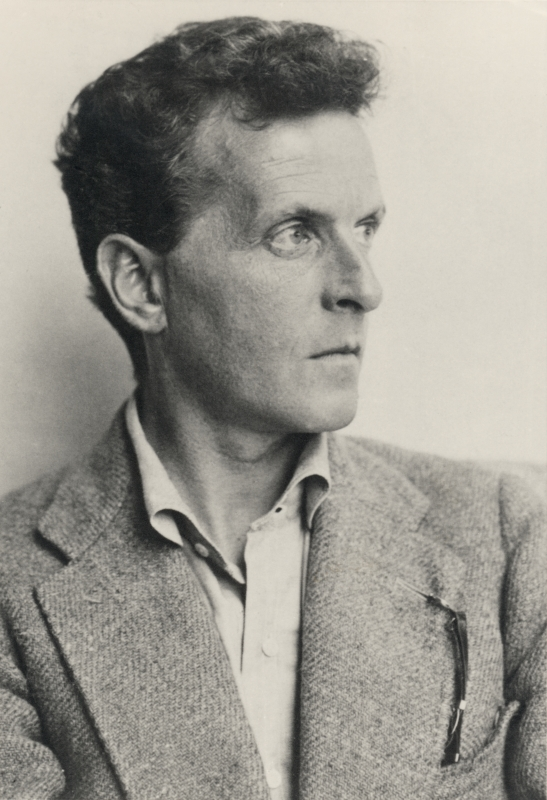
\includegraphics[scale=1.2]{material/Ludwig_Wittgenstein}
		\end{center}	
		\caption{Ludwig Wittgenstein (1930)}
	\end{figure}
	
\end{minipage}
~
\begin{minipage}{.65\textwidth}
	
	\begin{quote}
		4.025 Einen Satz verstehen, heißt, wissen \textbf{was der Fall ist}, wenn er wahr ist. (Man kann ihn also verstehen, \textbf{ohne zu wissen, ob er wahr ist}.) Man versteht ihn, wenn man seine \textbf{Bestandteile} versteht. 
	\end{quote}
	\hfill \citep{Wittgenstein72a}
	
\end{minipage}

\end{frame}


%%%%%%%%%%%%%%%%%%%%%%%%%%%%%%%%%%%%%%%%%%

\begin{frame}
\frametitle{Satzsemantik (Satzbedeutung)}

\begin{itemize}
	\item Die Bedeutung eines Satzes zu kennen, heißt also, \textbf{notwendige} und \textbf{hinreichende} Bedingungen für die Wahrheit bzw.\ Falschheit des Satzes ($=$ seine Wahrheitsbedingungen) zu kennen.
	\item[]
	\item Bedingungen in der aktuellen Welt (verschiedene Welten)
\end{itemize}

\pause 
	
	\ea Martin kauft Brötchen.
	\z
	
\begin{itemize}	
	\item Wahr oder Falsch (1 oder 0) \ras abhängig von der Welt
\end{itemize}

\pause 	
	
	\ea Verdaustig war's und glasse Wieben rotterten gorkicht im Gemank [\dots] \citep{SySt06a}.
	\z 
	


\end{frame}

%%%%%%%%%%%%%%%%%%%%%%%%%%%%%%%%%%%%%%%%%%

\begin{frame}
\frametitle{Satzsemantik (Satzbedeutung)}

\begin{block}{Kompositionalitätsprinzip}
Die Bedeutung eines komplexen Ausdrucks ergibt sich aus der \textbf{Bedeutung seiner unmittelbaren syntaktischen Teile} und der \textbf{Art und Weise}, wie sie sich syntaktisch \textbf{zusammensetzen}.
\end{block}

\begin{itemize}
	\item Auch Fregeprinzip genannt
\end{itemize}

\end{frame}


%%%%%%%%%%%%%%%%%%%%%%%%%%%%%%%%%%%%%%%%%%
%%%%%%%%%%%%%%%%%%%%%%%%%%%%%%%%%%%%%%%%%%
%
\subsubsection{Aussagenlogik}
%\frame{
%\begin{multicols}{2}
%\frametitle{~}
%	\tableofcontents[currentsection]
%\end{multicols}
%}
%%%%%%%%%%%%%%%%%%%%%%%%%%%%%%%%%%%%%%%%%%
\begin{frame}
\frametitle{Aussagenlogik}

\begin{itemize}
	\item basierend auf dem Kompositionalitätsprinzip
	\item[]
	\item Teilgebiet der formalen Logik
	\item[]
	\item Wie lässt sich der \textbf{Wahrheitswert einer komplexen Aussage} aus den Wahrheitswerten der in ihr enthaltenen \textbf{einfachen Aussagen} in Abhängigkeit der Verknüpfung errechnen?
\end{itemize}

\end{frame}


%%%%%%%%%%%%%%%%%%%%%%%%%%%%%%%%%%%%%%%%%%
\begin{frame}
\begin{minipage}{.67\textwidth}
	
	\begin{itemize}
		\item \textbf{Aussagenlogik:} Teil der formalen Logik, die sich mit der Bedeutung von Sätzen/Aussagen und ihrer Kombinatorik befasst
		\item[] 
		\item nach Aristoteles: Eine \textbf{Aussage} ist etwas, von dem man sagen kann, dass es \textbf{wahr} oder \textbf{falsch} ist.
		
	\end{itemize}	
	
	\begin{block}{Logik (Schlussfolgerungslehre)}
		Sie untersucht die \textbf{Struktur von Argumenten} im Hinblick auf ihre Gültigkeit anhand einer \textbf{künstlichen Sprache}, die im Vgl. zur natürlichen Sprache \textbf{weder ambig noch vage} ist.
	\end{block}
	
\end{minipage}
%%
\begin{minipage}{.30\textwidth}
	\begin{figure}
		\begin{center}
			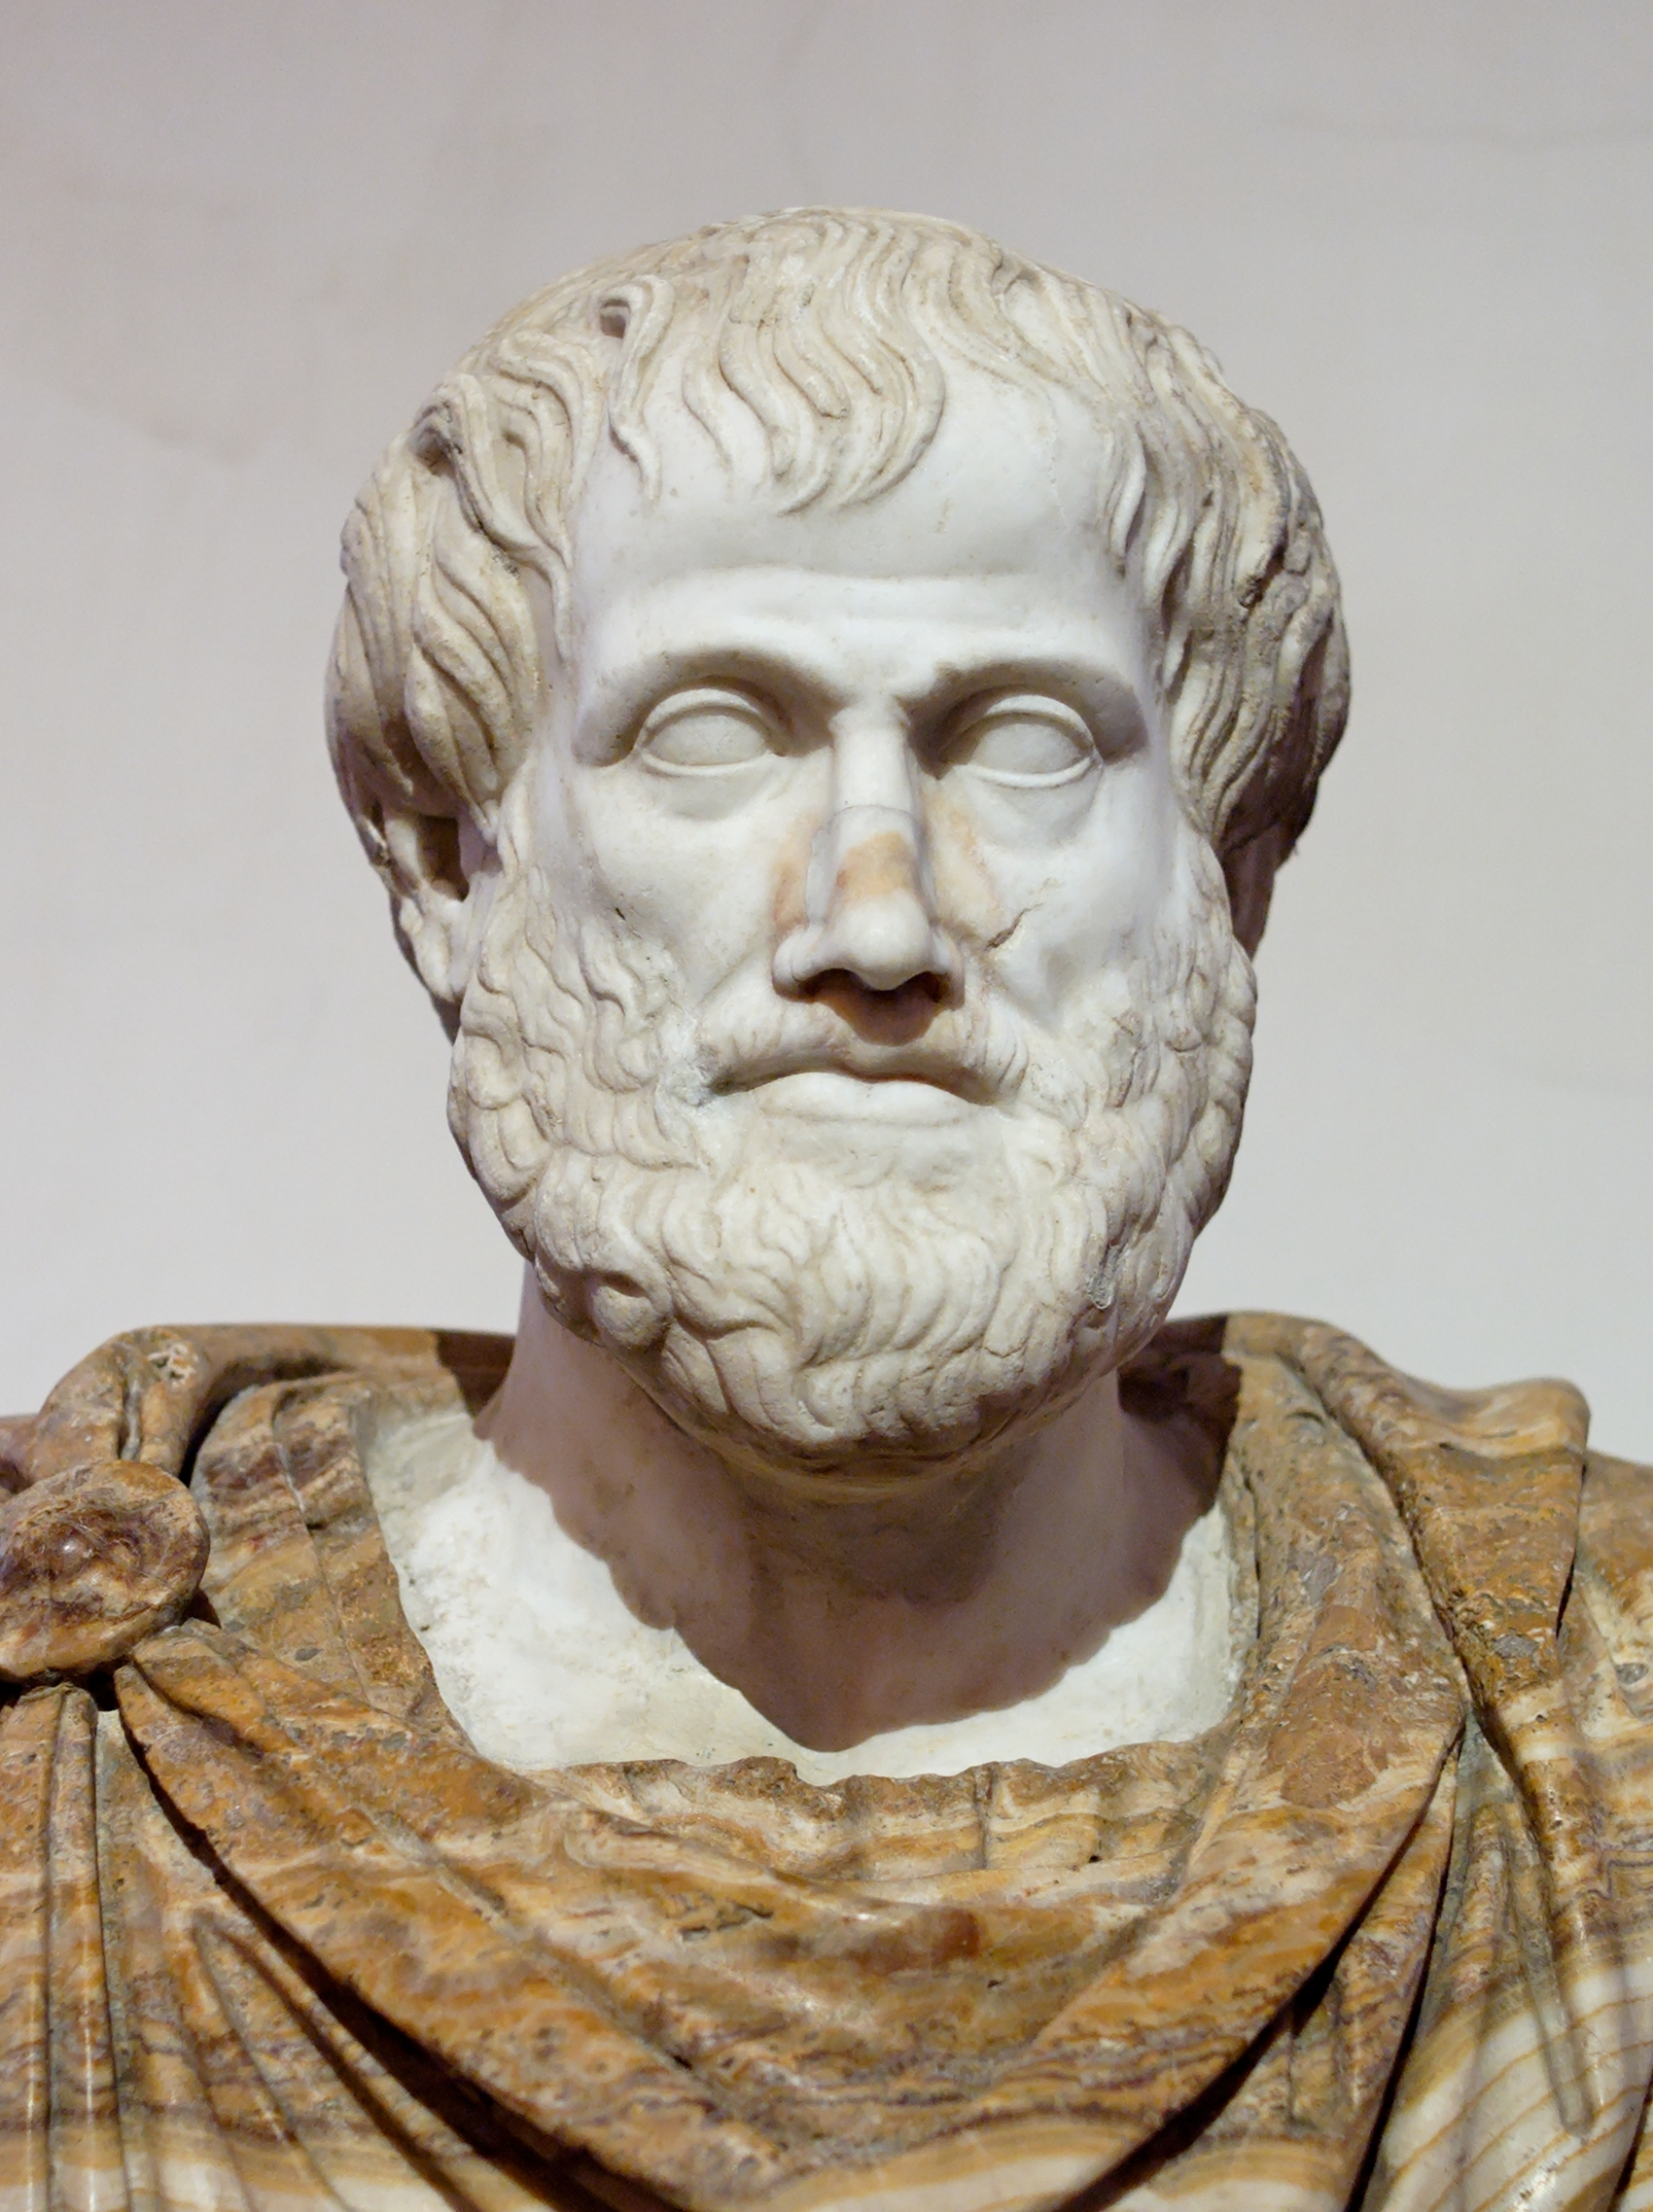
\includegraphics[scale=.45]{material/Aristotle_Altemps}
		\end{center}	
		\caption{Aristoteles}
	\end{figure}
\end{minipage}

\end{frame}

%%%%%%%%%%%%%%%%%%%%%%%%%%%%%%%%%%%%%%%%%%

\begin{frame}
\frametitle{Aussagenlogik}

\begin{itemize}
	\item Aussagen: p, q, r, s, \dots
	\item[]
	\item Konnektoren:
	
	\begin{itemize}
		\item Negation (NICHT): $\lnot$
		\item[]
		\item Konjunktion (UND): $\land$
		\item[]
		\item Disjunktion (UND/ODER): $\lor$
		\item[]
		\item Konditional (materiale Implikation) (WENN, DANN): \ras
		\item[]
		\item Bikonditional (GENAU DANN WENN): $\leftrightarrow$
	\end{itemize}
	
\end{itemize}

\end{frame}


%%%%%%%%%%%%%%%%%%%%%%%%%%%%%%%%%%%%%%%%%%

\begin{frame}
\frametitle{Aussagenlogik}

\begin{itemize}
	\item Negation (NICHT): $\lnot$
	
	\eal
		\ex $p$: Es regnet.
		\ex $\lnot p$: Es regnet nicht.
	\zl
	
\end{itemize}

\begin{table}
\centering
\begin{tabular}{p{3cm}|p{3cm}}
\textbf{p} & \textbf{$\lnot$p}\\
\hline
1 & 0\\
\hline
0 & 1\\
\end{tabular}
\end{table}

\end{frame}


%%%%%%%%%%%%%%%%%%%%%%%%%%%%%%%%%%%%%%%%%%

\begin{frame}
\frametitle{Aussagenlogik}

\begin{itemize}
	\item Konjunktion (UND): $\land$
	
	\eal
		\ex $p$: Es regnet.
		\ex $q$: Es donnert.
		\ex $p \land q$: Es regnet und es donnert.
	\zl

\end{itemize}
	

\begin{table}
\centering

\begin{tabular}{p{2cm}|p{2cm}|p{2cm}}
\textbf{p} & \textbf{q} & \textbf{p} $\land$ \textbf{q}\\
\hline
1 & 1 & 1\\
\hline
1 & 0 & 0\\
\hline
0 & 1 & 0\\
\hline 
0 & 0 & 0\\
\end{tabular}

\end{table}	

\end{frame}


%%%%%%%%%%%%%%%%%%%%%%%%%%%%%%%%%%%%%%%%%%

\begin{frame}
\frametitle{Aussagenlogik}

\begin{itemize}
	\item Disjunktion (UND/ODER): $\lor$

	\eal
		\ex $p$: Es regnet.
		\ex $q$: Es schneit.
		\ex $p \lor q$: Es regnet oder es schneit.
	\zl

\end{itemize}


\begin{table}
\centering

\begin{tabular}{p{2cm}|p{2cm}|p{2cm}}
\textbf{p} & \textbf{q} & \textbf{p} $\lor$ \textbf{q}\\
\hline
1 & 1 & 1\\
\hline
1 & 0 & 1\\
\hline
0 & 1 & 1\\
\hline 
0 & 0 & 0\\
\end{tabular}

\end{table}		

\end{frame}


%%%%%%%%%%%%%%%%%%%%%%%%%%%%%%%%%%%

\begin{frame}
\frametitle{Aussagenlogik}

\begin{itemize}
	\item Konditional (materiale Implikation) (WENN, DANN): \ras
	
	\eal
		\ex $p$: Es regnet.
		\ex $q$: Die Stra\ss{}e ist nass.
		\ex $p \rightarrow q$ : Wenn es regnet, dann ist die Stra\ss{}e nass.
	\zl

\end{itemize}

\begin{table}
\centering
\begin{tabular}{p{2cm}|p{2cm}|p{2cm}}
\textbf{p} & \textbf{q} & \textbf{p} \ras \textbf{q}\\
\hline
1 & 1 & 1\\
\hline
1 & 0 & 0\\
\hline
0 & 1 & 1\\
\hline 
0 & 0 & 1\\
\end{tabular}
\end{table}	


\end{frame}


%%%%%%%%%%%%%%%%%%%%%%%%%%%%%%%%%%%

\begin{frame}
\frametitle{Aussagenlogik}

\begin{itemize}
	\item Bikonditional (GENAU DANN WENN): $\leftrightarrow$
	
	\eal
		\ex $p$: Peter raucht.
		\ex $q$: Maria trinkt.
		\ex $p \leftrightarrow q$: Genau dann wenn Peter raucht, trinkt Maria.
	\zl

\end{itemize}


\begin{table}
\centering

\begin{tabular}{p{2cm}|p{2cm}|p{2cm}}
\textbf{p} & \textbf{q} & \textbf{p} $\leftrightarrow$ \textbf{q}\\
\hline
1 & 1 & 1\\
\hline
1 & 0 & 0\\
\hline
0 & 1 & 0\\
\hline 
0 & 0 & 1\\
\end{tabular}

\end{table}

\end{frame}


%%%%%%%%%%%%%%%%%%%%%%%%%%%%%%%%%%%%%%%%%%
%%%%%%%%%%%%%%%%%%%%%%%%%%%%%%%%%%%%%%%%%%
%
\subsubsection{Übung}
%\frame{
%\begin{multicols}{2}
%\frametitle{~}
%	\tableofcontents[currentsection]
%\end{multicols}
%}
%%%%%%%%%%%%%%%%%%%%%%%%%%%%%%%%%%%%%%%%%%

%%%%%%%%%%%%%%%%%%%%%%%%%%%%%%%%%%%%
%%%%%%%%%%%%%%%%%%%%%%%%%%%%%%%%%%%%
%\iftoggle{uebung}{
%%%%%%%%%%%%%%%%%%%%%%%%%%%%%%%%%%%%%
%\begin{frame}
%\frametitle{Aussagenlogik -- Übung}
%
%\begin{itemize}
%	\item Geben Sie die folgenden Aussagen in aussagenlogischer Notation an:
%\end{itemize}
%
%\ea Christiane schläft.
%\ex Norbert raucht nicht.
%\ex Norbert raucht und Christiane schläft nicht.
%\ex Wenn Norbert nicht raucht, schläft Christiane nicht.
%\ex Wenn ich schlafe, träume ich.
%\ex Ich schlafe nicht oder ich träume.
%\z 
%
%\end{frame}
%
%} 
%%% END uebung true = Q
%%% BEGIN uebung false = A
%{
%%%%%%%%%%%%%%%%%%%%%%%%%%%%%%%%%%%%
\begin{frame}
\frametitle{Aussagenlogik -- Übung}

\begin{itemize}
	\item Geben Sie die folgenden Aussagen in aussagenlogischer Notation an.
\end{itemize}

\ea\label{ex:Form1} Christiane schläft. 
\ex\label{ex:Form2} Norbert raucht nicht. 
\ex\label{ex:Form3} Norbert raucht und Christiane schläft nicht. 
\ex\label{ex:Form4} Wenn Norbert nicht raucht, schläft Christiane nicht. 
\ex\label{ex:Form5} Wenn ich schlafe, träume ich. 
\ex\label{ex:Form6} Ich schlafe nicht oder ich träume.
\z 

\end{frame}

%%%%%%%%%%%%%%%%%%%%%%%%%%%%%%%%%%%%
\iftoggle{ue-loesung}{

	%%%%%%%%%%%%%%%%%%
%Lösung Semantik 
%%%%%%%%%%%%%%%%%%


\begin{frame}
\frametitle{Übung -- Lösung}

\begin{itemize}
	\item Geben Sie die folgenden Aussagen in aussagenlogischer Notation an:
\end{itemize}

\begin{exe}
	\exr{ex:Form1} Christiane schläft. \hfill \alertgreen{$p$}
	\exr{ex:Form2} Norbert raucht nicht. \hfill \alertgreen{$\lnot p$}
	\exr{ex:Form3} Norbert raucht und Christiane schläft nicht. \hfill \alertgreen{$(p \land \lnot q)$}
	\exr{ex:Form4} Wenn Norbert nicht raucht, schläft Christiane nicht. \hfill \alertgreen{$(\lnot p \rightarrow \lnot q)$}
	\exr{ex:Form5} Wenn ich schlafe, träume ich. \hfill \alertgreen{$(p \rightarrow q)$}
	\exr{ex:Form6} Ich schlafe nicht oder ich träume. \hfill \alertgreen{$(\lnot p \lor q)$}
\end{exe}

\end{frame}

	
}
%%%%%%%%%%%%%%%%%%%%%%%%%%%%%%%%%%%%
%\iftoggle{uebung}{
%%%%%%%%%%%%%%%%%%%%%%%%%%%%%%%%%%%%	
%\begin{frame}
%\frametitle{Aussagenlogik -- Übung}
%
%\begin{itemize}
%	\item Geben Sie die Wahrheitswertetabellen für die folgenden Aussagen an:
%\end{itemize}
%
%\ea Christiane schläft.
%\ex Norbert raucht nicht.
%\ex Norbert raucht und Christiane schläft nicht.
%\ex Wenn Norbert nicht raucht, schläft Christiane nicht.
%\ex Wenn ich schlafe, träume ich.
%\ex Ich schlafe nicht oder ich träume.
%\z 
%
%\end{frame}
%} 
%%% END uebung true = Q
%%% BEGIN uebung false = A
%{
%%%%%%%%%%%%%%%%%%%%%%%%%%%%%%%%%%%%	

\begin{frame}
\frametitle{Aussagenlogik -- Übung}

\begin{itemize}
	\item Geben Sie die Wahrheitswertetabellen für die folgenden Aussagen an:
\end{itemize}

\ea\label{ex:AL1} Christiane schläft.
\ex\label{ex:AL2} Norbert raucht nicht.
\ex\label{ex:AL3} Norbert raucht und Christiane schläft nicht.
\ex\label{ex:AL4} Wenn Norbert nicht raucht, schläft Christiane nicht.
\ex\label{ex:AL5} Wenn ich schlafe, träume ich.
\ex\label{ex:AL6} Ich schlafe nicht oder ich träume.
\z 

\end{frame}


%%%%%%%%%%%%%%%%%%%%%%%%%%%%%%%%%%%%%%%%%%
\iftoggle{ue-loesung}{

%%%%%%%%%%%%%%%%%%%%%%%
%Semantik 07 ue-loesung03
%%%%%%%%%%%%%%%%%%%%%%%


\begin{frame}
\frametitle{Übung -- Lösung}

\begin{exe}
\exr{ex:AL1} Christiane schläft.
\exr{ex:AL2} Norbert raucht nicht.
\end{exe}

\begin{minipage}{0.4\textwidth}
	\centering
	\begin{itemize}
		\item[] \small{p: Christiane schläft.}
	\end{itemize}
	\scalebox{0.8}{
		\begin{tabular}{l}
			p\\
			\hline
			1\\
			\hline
			0\\
		\end{tabular}
	}
\end{minipage}
%	
\begin{minipage}{0.5\textwidth}
	\centering
	\begin{itemize}
		\item[] \small{p: Norbert raucht.}
	\end{itemize}
	\scalebox{0.8}{
		\begin{tabular}[b]{l|l}
			p & $ \lnot $p \\
			\hline
			0 & 1 \\
			\hline
			1 & 0 \\
	\end{tabular}
	}

\end{minipage}
\end{frame}


%%%%%%%%%%%%%%%%%%%%%%%%%%%%%%%%%%%	
\begin{frame}
\frametitle{Übung -- Lösung}

\begin{exe}
	\exr{ex:AL3} Norbert raucht und Christiane schläft nicht.
	\exr{ex:AL4} Wenn Norbert nicht raucht, schläft Christiane nicht.
\end{exe}

\begin{minipage}{0.45\textwidth}
	\centering
	\begin{itemize}
		\item[] \small{p: Norbert raucht.\\
			q: Christiane schläft.}
	\end{itemize}
	\scalebox{0.8}{
		\begin{tabular}{l|l|l|c}
			p & q & $\lnot$ q & p $\land \lnot $q\\
			\hline
			1 & 1 & 0 & 0\\
			\hline
			1 & 0 & 1 & 1\\
			\hline
			0 & 1 & 0 & 0 \\
			\hline
			0 & 0 & 1 & 0 \\
		\end{tabular}
	}
\end{minipage}
%%
%%
\begin{minipage}{0.5\textwidth}
	\centering
	\begin{itemize}
		\item[] \small{p: Norbert raucht.\\
			q: Christiane schläft.}
	\end{itemize}
	\scalebox{0.8}{
		\begin{tabular}{l|l|c|c|c}
			p & q & $ \lnot $p& $ \lnot $q &$ \lnot $p \ras $ \lnot $q\\
			\hline
			1 & 1 & 0 & 0 & 1 \\
			\hline
			1 & 0 & 0 & 1 & 1\\
			\hline
			0 & 1 & 1 & 0 & 0 \\
			\hline
			0 & 0 & 1 & 1 & 1 \\
	\end{tabular}
	}
\end{minipage}

\end{frame}


%%%%%%%%%%%%%%%%%%%%%%%%%%%%%%%%%%%	
\begin{frame}
\frametitle{Übung -- Lösung}

\begin{exe}
	\exr{ex:AL5} Wenn ich schlafe, träume ich.
	\exr{ex:AL6} Ich schlafe nicht oder ich träume.
\end{exe}


\begin{minipage}{0.48\textwidth}
\centering
\begin{itemize}
	\item[] \small{$p$: Ich schlafe.\\
	$q$: Ich träume.}
\end{itemize}

\scalebox{0.8}{
\begin{tabular}[b]{c|c|c}
	$p$ & $q$ & $p \ras q$ \\
	\hline
	1 & 1 & 1 \\
	\hline
	1 & 0 & 0 \\
	\hline
	0 & 1 & 1 \\
	\hline
	0 & 0 & 1 \\
\end{tabular}}
\end{minipage}
%%
%%
\begin{minipage}{0.48\textwidth}
\centering
\begin{itemize}
	\item[] \small{p: Ich schlafe.\\
	q: Ich träume.}
\end{itemize}

\scalebox{0.8}{
\begin{tabular}{c|c|c|c}
	$p$ & $q$ & $\lnot p$ & $ \lnot p \lor q$\\
	\hline
	1 & 1 & 0 & 1 \\
	\hline
	1 & 0 & 0 & 0 \\
	\hline
	0 & 1 & 1 & 1 \\
	\hline
	0 & 0 & 1& 1 \\
\end{tabular}}
\end{minipage}

\end{frame}

}
%%%%%%%%%%%%%%%%%%%%%%%%%%%%%%%%%%%%%%%%%%
%
\subsubsection{Tautologien, Kontradiktionen, Kontingenzen}
%\frame{
%\begin{multicols}{2}
%\frametitle{~}
%	\tableofcontents[currentsection]
%\end{multicols}
%}
%%%%%%%%%%%%%%%%%%%%%%%%%%%%%%%%%%%%%%%%%%

\begin{frame}{Tautologien, Kontradiktionen, Kontingenzen}

\begin{itemize}
	\item (komplexe) Aussagen, deren Wahrheitswert  \textbf{nicht vom Wahrheitswert der Teilaussagen abhängig} ist: \textbf{Tautologien} und \textbf{Kontradiktionen} 
	
	\item[]
	
	\item (komplexe) Aussagen, deren Wahrheitswert \textbf{vom Wahrheitswert der Teilaussagen abhängig} ist: \textbf{Kontingenzen} 
	
\end{itemize}

\end{frame}


%%%%%%%%%%%%%%%%%%%%%%%%%%%%%%%%%%%
\begin{frame}{Tautologie}

\begin{itemize}
	\item \textbf{logische Wahrheit} (aufgrund der Ausdrucksbedeutung)
\end{itemize}

\begin{block}{Tautologie}
	Von Wittgenstein in die formale Logik eingeführter Terminus für Aussagen, die aufgrund ihrer semantischen Form analytisch und darum \textbf{in allen möglichen Welten wahr} sind \citep{Rehbock16a}
\end{block}

\ea Frösche sind Amphibien. 
\ex Wir verstehen Semantik oder wir verstehen Semantik nicht.
\z 

\pause 

\begin{table}
	\centering	
	%	\scalebox{0.8}{
	\begin{tabular}{c|c|c}
		\textbf{p}& \textbf{$\lnot$p} &\textbf{(p$\lor \lnot$p)} \\ 
		\hline 
		1 & 0 & \alertred{1}\\ 
		\hline 
		0 & 1 & \alertred{1}		
		
	\end{tabular} 
	%	}
\end{table}

\end{frame}


%%%%%%%%%%%%%%%%%%%%%%%%%%%%%%%%%%%
\begin{frame}{Kontradiktion}

\begin{itemize}
	\item \textbf{logische Falschheit} (aufgrund der Ausdrucksbedeutung)
\end{itemize}

\begin{block}{Kontradiktion}
	Logischer Terminus für Aussagen, die aufgrund ihrer semantischen Form \textbf{in allen möglichen Welten falsch} sind \citep{Rehbock16b}
\end{block}

\ea Frösche sind Reptilien. 
\ex Die Sonne scheint, aber sie scheint nicht.
\z 

\pause

\begin{table}
	\centering	
	%	\scalebox{0.8}{
	\begin{tabular}{c|c|c}
		\textbf{p}& \textbf{$\lnot$p} &\textbf{(p$\land \lnot$p)} \\ 
		\hline 
		1 & 0 & \alertred{0}\\ 
		\hline 
		0 & 1 & \alertred{0}		
		
	\end{tabular} 
	%	}
\end{table}

\begin{itemize}
	\item Beide Teilaussagen können nicht gleichzeitig wahr sein.
\end{itemize}

\end{frame}


%%%%%%%%%%%%%%%%%%%%%%%%%%%%%%%%%%%
\begin{frame}{Kontingenz}

\begin{block}{(logische) Kontingenz}
	Eine Aussage ist logisch kontingent, \textbf{wenn deren gegenteilige Aussage keinen Widerspruch einschließt}; ein Satz ist logisch kontingent, wenn er weder in seiner positiven noch in seiner negativen Bestimmung notwendig logisch wahr ist. Ein kontingenter Satz ist \textbf{logisch wahr in einigen, nicht aber in allen  möglichen Welten} (semantische Deutung) [\dots] \citep{Prechtl16b}.
\end{block}

\ea Wir lieben Semantik und wir hassen Pragmatik.
\z 

\pause 

\begin{table}
	\centering	
	\scalebox{0.7}{
		\begin{tabular}{c|c|c}
			\textbf{p}& \textbf{q} &\textbf{(p$\land$q)} \\ 
			\hline 
			1 & 1 & \alertred{1}\\ 
			\hline 
			1 & 0 & \alertred{0}\\ 
			\hline 
			0 & 1 & \alertred{0}\\ 
			\hline 
			0 & 0 & \alertred{0}				
			
		\end{tabular} 
	}
\end{table} 

\end{frame}


%%%%%%%%%%%%%%%%%%%%%%%%%%%%%%%%%%%%
%\begin{frame}
%\frametitle{Aussagenlogik}
%
%\begin{itemize}
%	\item \textbf{Tautologie}
%	
%	\begin{itemize}
%		\item Aussage, die stets wahr ist (unabhängig von den
%Ausgangswerten der beteiligten Aussagen)
%		
%		\ea Es regnet oder es regnet nicht.
%		\z
%		
%	\end{itemize}
%	
%	\item \textbf{Kontradiktion}
%	
%	\begin{itemize}
%		\item  Aussage, die stets falsch ist (unabhängig von den
%Ausgangswerten der beteiligten Aussagen)
%
%		\ea Es regnet und es regnet nicht.
%		\z
%		
%	\end{itemize}
%	
%	\item \textbf{Kontigenz}
%	
%	\begin{itemize}
%		\item Aussage, die abhängig von den Ausgangswerten der beteiligten Aussage sowohl wahr als auch falsch sein kann.
%
%		\ea Es regnet oder es schneit.
%		\z
%
%	\end{itemize}
%	
%\end{itemize}
%
%\end{frame}


%%%%%%%%%%%%%%%%%%%%%%%%%%%%%%%%%%%
%%%%%%%%%%%%%%%%%%%%%%%%%%%%%%%%%%%

%%%%%%%%%%%%%%%%%%%%%%%%%%%%%%%%%%%
\begin{frame}
\frametitle{Tautologien, Kontradiktionen, Kontingenzen -- Übung}

\begin{itemize}
	\item Überprüfen Sie die Richtigkeit der folgenden Aussagen.
	
	\vspace{1em}
	
	\begin{itemize}
		\item Die komplexen Aussagen (\ref{ex:Tau1}) und (\ref{ex:Tau2}) sind \textbf{Tautologien}.
	
		\ea
			\ea\label{ex:Tau1} (p $\lor \lnot$ p)
			\ex\label{ex:Tau2} (p $\rightarrow$ p)
			\z 
		\z
			
		\item Die komplexe Aussagen (\ref{ex:Kon1}) ist eine \textbf{Kontradiktion}.
		
		\ea
			\ea\label{ex:Kon1} $\lnot$ (p $\lor \lnot$ p)
			\z 
		\z

		\item Die komplexe Aussage (\ref{ex:Con1}) ist eine \textbf{Kontingenz}.
		
		\ea
			\ea\label{ex:Con1} ((p $\lor$ q) $\rightarrow$ q)
			\z
		\z
			
	\end{itemize}	
	
\end{itemize}

\end{frame}



%%%%%%%%%%%%%%%%%%%%%%%%%%%%%%%%%
\iftoggle{ue-loesung}{

%%%%%%%%%%%%%%%%%%%%%%%%
%Semantik 07-ue-loesung04
%%%%%%%%%%%%%%%%%%%%%%%%%


\begin{frame}
\frametitle{Übung -- Lösung}

\begin{itemize}
	\item Überprüfen Sie die Richtigkeit der folgenden Aussagen.
	
	\begin{itemize}
		\item Die komplexen Aussagen (\ref{ex:Tau1}) und (\ref{ex:Tau2}) sind \textbf{Tautologien}.
		
		\begin{exe}
		\exr{ex:Tau1} (p $\lor \lnot$ p)
		\exr{ex:Tau2} (p $\rightarrow$ p)
		\end{exe}
		
	\end{itemize}
\end{itemize}

\begin{table}
	\centering	
	%	\scalebox{0.8}{
	\begin{tabular}{c|c|c}
		\textbf{p}& \textbf{$\lnot$p} &\textbf{(p $\lor \lnot$p)} \\ 
		\hline 
		1 & 0 & \alertred{1}\\ 
		\hline 
		0 & 1 & \alertred{1} \\
	\end{tabular} 
	%	}
\end{table}
\begin{itemize}
	\item[]  \alertred{Der Satz ist eine Tautologie, weil die Aussage immer wahr ist (immer Wahrheitswert 1).}
\end{itemize}

\end{frame}


%%%%%%%%%%%%%%%%%%%%%%%%%%%%%%%%%%
\begin{frame}
\frametitle{Übung -- Lösung}

\begin{itemize}
	\item Überprüfen Sie die Richtigkeit der folgenden Aussagen.
	
	\begin{itemize}
		\item Die komplexe Aussagen (\ref{ex:Kon1}) ist eine \textbf{Kontradiktion}.
		
		\begin{exe}
		\exr{ex:Kon1} $\lnot$ (p $\lor \lnot$ p)
		\end{exe}
		
	\end{itemize}	
	
\end{itemize}

\begin{table}
	\centering	
	%	\scalebox{0.8}{
	\begin{tabular}{c|c|c|c}
		\textbf{p}& \textbf{$\lnot$p} &\textbf{(p $\lor \lnot$p)} & $\lnot$ \textbf{(p $\lor \lnot$p)}\\ 
		\hline 
		1 & 0 & 1& \alertred{0} \\ 
		\hline 
		0 & 1 & 1 & \alertred{0} \\
	\end{tabular} 
	%	}
\end{table}
\begin{itemize}
	\item[] \alertred{Der Satz ist ein Kontradiktion, weil der Wahrheitswert immer 0 ist. Die Aussage ist immer falsch.}
\end{itemize}

\end{frame}


%%%%%%%%%%%%%%%%%%%%%%%%%%%%%%%%%%
\begin{frame}
\frametitle{Übung -- Lösung}

\begin{itemize}
	\item Überprüfen Sie die Richtigkeit der folgenden Aussagen.
	
	\begin{itemize}
		\item Die komplexe Aussage (\ref{ex:Con1}) ist eine \textbf{Kontingenz}.
		
		\begin{exe}
		\exr{ex:Con1} ((p $\lor$ q) $\rightarrow$ q)
		\end{exe}
		
	\end{itemize}	
	
\end{itemize}

\begin{table}
	\centering	
	%	\scalebox{0.8}{
	\begin{tabular}{c|c|c|c}
		\textbf{p}& \textbf{q} & \textbf{(p $\lor$ q)} & \textbf{(p $\lor$ q) \ras q}\\ 
		\hline 
		1 & 0 & 1& \alertred{0} \\ 
		\hline 
		1 & 1 & 1 & \alertred{1} \\
		\hline 
		0 & 0 & 0 & \alertred{1}\\
		\hline 
		0 & 1 &  1 &  \alertred{1}\\
	\end{tabular} 
	%	}
\end{table}

\begin{itemize}
\item \alertred{Der Satz ist kontingent, d.\,h., dass sich unterschiedliche Wahrheitwerte ergeben können, die von der Welt abhängig sind. }
\end{itemize}

\end{frame}

}
%%%%%%%%%%%%%%%%%%%%%%%%%%%%%%%%%%%


%%%%%%%%%%%%%%%%%%%%%%%%%%%%%%%%%%%
%%%%%%%%%%%%%%%%%%%%%%%%%%%%%%%%%%%
\subsubsection{(Einige) Äquivalenzen -- Extra}
%\frame{
%\begin{multicols}{2}
%\frametitle{~}
%	\tableofcontents[currentsection]
%\end{multicols}
%}
%%%%%%%%%%%%%%%%%%%%%%%%%%%%%%%%%%%

\begin{frame}
\frametitle{(Einige) Äquivalenzen -- Extra}

\begin{itemize}
	\item Einige komplexe aussagenlogische Formeln sind formal unterschiedlich, zeigen jedoch die gleichen Wahrheitswerte unter den gleichen Wahrheitsbedingungen (d.\,h. in den gleichen Welten). 

	\item Solche Formeln nennt man \textbf{äquivalent}. 
	
	\item Es gibt mehrere komplexe aussagenlogische Formeln, die äquivalent sind. Man kennt sie unter dem Namen \alertred{aussagenlogische Gesetze} (\textit{Laws of statement logic})  \citep[vgl.][]{Partee&Co93a}.
	
	\item Genau dann wenn zwei komplexe Aussagen äquivalent sind, ist deren Verbindung mittels eines Bikonditionalen eine \textbf{Tautologie}.

\end{itemize}


\end{frame}


%%%%%%%%%%%%%%%%%%%%%%%%%%%%%%%%%%%
\begin{frame}
%\frametitle{Bikonditional}

Geben Sie die Wahrheitswerte für die folgenden komplexen Aussagen an und vergleichen Sie die Ergebnisse beider Tabellen.

\ea\label{ex:Equi1} Genau dann wenn ich Durst habe, trinke ich Wasser.

\ex\label{ex:Equi2} Es ist nicht der Fall, dass ich Durst habe, und es ist nicht der Fall, dass ich Wasser trinke -- oder -- es ist der Fall, dass ich Durst habe und es ist der Fall, dass ich Wasser trinke.
\z 

\end{frame}


%%%%%%%%%%%%%%%%%%%%%%%%%%%%%%%%%%%
\begin{frame}
%\frametitle{Bikonditional}

\begin{exe}
\exr{ex:Equi1} Genau dann wenn ich Durst habe, trinke ich Wasser.

\exr{ex:Equi2} Es ist nicht der Fall, dass ich Durst habe, und es ist nicht der Fall, dass ich Wasser trinke -- oder -- es ist der Fall, dass ich Durst habe und es ist der Fall, dass ich Wasser trinke.
\end{exe}


{\small $p$: Ich habe Durst.\\
$q$: Ich trinke Wasser.}

\pause 

\begin{minipage}{0.35\textwidth}
	\centering

	\scalebox{0.7}{
		\begin{tabular}{c|c|c}
			$p$ & $q$ & $p \leftrightarrow q$\\
			\hline
			1 & 1 & \alertred{1}\\
			\hline
			1 & 0 & \alertred{0}\\
			\hline
			0 & 1 & \alertred{0}\\
			\hline
			0 & 0 & \alertred{1}\\
		\end{tabular}
	}
\end{minipage}
%%
\pause
%%	
\begin{minipage}{0.55\textwidth}
	\centering

	\scalebox{0.7}{
		\begin{tabular}{c|c|c|c|c}
			$p$ & $q$ & $\lnot p \land \lnot q$ & $p \land q$ & $( \lnot p \land \lnot q) \lor (p \land q)$\\
			\hline
			1 & 1 & 0 & 1 & \alertred{1}\\
			\hline
			1 & 0 & 0 & 0 & \alertred{0}\\
			\hline
			0 & 1 & 0 & 0 & \alertred{0}\\
			\hline
			0 & 0 & 1 & 0 & \alertred{1}\\
	\end{tabular}}
\end{minipage}

\end{frame}


%%%%%%%%%%%%%%%%%%%%%%%%%%%%%%%%%%%
\begin{frame}
%\frametitle{Bikonditional}

Die komplexe Formeln $P$ und $Q$ sind \textbf{äquivalent} ($P \Leftrightarrow Q$), denn $P \leftrightarrow Q$ ist eine Tautologie. (Testen Sie dies!)

\begin{exe}

	\exr{ex:Equi1} $P := p \leftrightarrow q$
	
	Genau dann wenn ich Durst habe, trinke ich Wasser.
	
	\exr{ex:Equi2} $Q := ( \lnot p \land \lnot q) \lor (p \land q)$
	
	Es ist nicht der Fall, dass ich Durst habe, und es ist nicht der Fall, dass ich Wasser trinke -- oder -- es ist der Fall, dass ich Durst habe und es ist der Fall, dass ich Wasser trinke.
\end{exe}
	
Diese Äquivalenz ist eines der \alertred{Gesetze des Bikonditionals} in der Aussagenlogik.

\end{frame}


%%%%%%%%%%%%%%%%%%%%%%%%%%%%%%%%%%%
\begin{frame}
%\frametitle{Distributivität}

Geben Sie die Wahrheitswerte für die folgenden komplexen Aussagen an und vergleichen Sie die Ergebnisse beider Tabellen.

	
	\ea\label{ex:Equi3} Es regnet -- oder -- es scheint die Sonne und ich bin froh.
	\ex\label{ex:Equi4} Es regnet oder es scheint die Sonne -- und -- es regnet oder ich bin froh.
	\z 
	 	
\end{frame}


%%%%%%%%%%%%%%%%%%%%%%%%%%
\begin{frame}%[shrink=20]
%\frametitle{Distributivität}

\begin{exe}
\exr{ex:Equi3} Es regnet -- oder -- es scheint die Sonne und ich bin froh.
\exr{ex:Equi4} Es regnet oder es scheint die Sonne -- und -- es regnet oder ich bin froh.
\end{exe}

{\small 
	$p$: Es regnet.\\
	$q$: Es scheint die Sonne.\\
	$s$: Ich bin froh.}

\pause

\begin{minipage}{0.45\textwidth}
	\centering

	\scalebox{0.7}{
		\begin{tabular}{c|c|c|c|c}
			$p$ & $q$ & $s$ & $q \land s$ & $p \lor (q \land s)$ \\
			\hline
			1 & 1 & 1 & 1 & \alertred{1}\\
			\hline
			1 & 1 & 0 & 0 & \alertred{1}\\
			\hline
			1 & 0 & 1 & 0 & \alertred{1}\\
			\hline
			1 & 0 & 0 & 0 & \alertred{1}\\
			\hline
			0 & 1 & 1 & 1 & \alertred{1}\\
			\hline
			0 & 1 & 0 & 0 & \alertred{0}\\
			\hline
			0 & 0 & 1 & 0 & \alertred{0}\\
			\hline
			0 & 0 & 0 & 0 & \alertred{0}\\
		\end{tabular}
	}
\end{minipage}
%%
\pause
%%
\begin{minipage}{0.5\textwidth}
	\centering

	\scalebox{0.7}{
		\begin{tabular}[b]{c|c|c|c|c|c}
			$p$ & $q$ & $s$ & $p \lor q$ & $p \lor s$ & $(p \lor q) \land (p \lor s)$ \\
			\hline
			1 & 1 & 1 & 1 & 1 & \alertred{1}\\
			\hline
			1 & 1 & 0 & 1 & 1 & \alertred{1}\\
			\hline
			1 & 0 & 1 & 1 & 1 & \alertred{1}\\
			\hline
			1 & 0 & 0 & 1 & 1 & \alertred{1}\\
			\hline
			0 & 1 & 1 & 1 & 1 & \alertred{1}\\
			\hline
			0 & 1 & 0 & 1 & 0 & \alertred{0}\\
			\hline
			0 & 0 & 1 & 0 & 1 & \alertred{0}\\
			\hline
			0 & 0 & 0 & 0 & 0 & \alertred{0}\\
			
	\end{tabular}}
\end{minipage}

\end{frame}


%%%%%%%%%%%%%%%%%%%%%%%%%%%%%%%%%%%
\begin{frame}
%\frametitle{Distributivität}

Die komplexe Formeln $P$ und $Q$ sind \textbf{äquivalent} ($P \Leftrightarrow Q$), denn $P \leftrightarrow Q$ ist eine Tautologie. (Testen Sie dies!)

\begin{exe}
	
	\exr{ex:Equi3} $P := p \lor (q \land s)$
	
	Es regnet -- oder -- es scheint die Sonne und ich bin froh.
	
	\exr{ex:Equi4} $Q := (p \lor q) \land (p \lor s)$
	
	Es regnet oder es scheint die Sonne -- und -- es regnet oder ich bin froh.
\end{exe}

Diese Äquivalenz ist eines der \alertred{Distributivitätsgesetze} in der Aussagenlogik.

\end{frame}


%%%%%%%%%%%%%%%%%%%%%%%%%%%%%%%%%%%
\begin{frame}
%\frametitle{DeMorgan}

Geben Sie die Wahrheitswerte für die folgenden komplexen Aussagen an und vergleichen Sie die Ergebnisse beider Tabellen.

\ea\label{ex:Equi5} Es ist nicht der Fall, dass Norbert raucht oder Christiane schläft.
\ex\label{ex:Equi6} Es ist nicht der Fall, dass Norbert raucht -- und -- es ist nicht der Fall dass Christiane schläft.
\z 	

\end{frame}


%%%%%%%%%%%%%%%%%%%%%%%%%%%%%%%%%%%
\begin{frame}
%\frametitle{DeMorgan}

\begin{exe}
	\exr{ex:Equi5} Es ist nicht der Fall, dass Norbert raucht oder Christiane schläft.
	\exr{ex:Equi6} Es ist nicht der Fall, dass Norbert raucht -- und -- es ist nicht der Fall dass Christiane schläft.
\end{exe} 

{\small 
	$p$: Norbert raucht.\\
	$q$: Christiane schläft.
}

\pause 

\begin{minipage}{0.48\textwidth}
	\centering
	
	\scalebox{0.8}{
		\begin{tabular}{c|c|c|c}
			$p$ & $q$ & $p \lor q$ & $ \lnot  (p  \lor q)$\\
			\hline
			1 & 1 & 1 & \alertred{0} \\
			\hline
			1 & 0 & 1 & \alertred{0} \\
			\hline
			0 & 1 & 1 & \alertred{0} \\
			\hline
			0 & 0 & 0 & \alertred{1} \\
	\end{tabular}}
\end{minipage}
%%
\pause
%%
\begin{minipage}{0.48\textwidth}
	\centering
	
	\scalebox{0.8}{
	\begin{tabular}{c|c|c|c|c}
		$p$ & $q$ & $\lnot p$ & $\lnot q$ & $(\lnot p \land \lnot q)$\\
		\hline
		1 & 1 & 0 & 0 & \alertred{0}\\
		\hline
		1 & 0 & 0 & 1 & \alertred{0}\\
		\hline
		0 & 1 & 1 & 0 & \alertred{0}\\
		\hline
		0 & 0 & 1 & 1 & \alertred{1}\\
	\end{tabular}}

\end{minipage}

\end{frame}


%%%%%%%%%%%%%%%%%%%%%%%%%%%%%%%%%%%
\begin{frame}
%\frametitle{DeMorgan}

Die komplexe Formeln $P$ und $Q$ sind \textbf{äquivalent} ($P \Leftrightarrow Q$), denn $P \leftrightarrow Q$ ist eine Tautologie. (Testen Sie dies!)

\begin{exe}
	
	\exr{ex:Equi5} $P := \lnot (p \lor q)$

	Es ist nicht der Fall, dass Norbert raucht oder Christiane schläft.
	
	\exr{ex:Equi6} $Q := (\lnot p \land \lnot q)$
	
	Es ist nicht der Fall, dass Norbert raucht -- und -- es ist nicht der Fall dass Christiane schläft.	

\end{exe}

Diese Äquivalenz ist eines der \alertred{DeMorgans Gesetze} in der Aussagenlogik.

\end{frame}


%%%%%%%%%%%%%%%%%%%%%%%%%%%%%%%%%%%
\begin{frame}
%\frametitle{Konditional}

Geben Sie die Wahrheitswerte für die folgenden komplexen Aussagen an und vergleichen Sie die Ergebnisse beider Tabellen:

\ea\label{ex:Equi7} Wenn ich schlafe, träume ich.
\ex\label{ex:Equi8} Ich schlafe nicht oder ich träume.
\z 	

\end{frame}

%%%%%%%%%%%%%%%%%%%%%%%%%
\begin{frame}
%\frametitle{Konditional}

\begin{exe}
	\exr{ex:Equi7} Wenn ich schlafe, träume ich.
	\exr{ex:Equi8} Ich schlafe nicht oder ich träume.
\end{exe}

{\small 
	$p$: Ich schlafe.\\
	$q$: Ich träume.
}

\pause 

\begin{minipage}{0.48\textwidth}
\centering

\scalebox{0.8}{
	\begin{tabular}{c|c|c}
		$p$ & $q$ & $p \rightarrow q$\\
		\hline
		1 & 1 & \alertred{1} \\
		\hline
		1 & 0 & \alertred{0} \\
		\hline
		0 & 1 & \alertred{1} \\
		\hline
		0 & 0 & \alertred{1} \\
\end{tabular}}
\end{minipage}
%%
\pause
%%
\begin{minipage}{0.48\textwidth}
\centering

\scalebox{0.8}{
\begin{tabular}{c|c|c|c}
	$p$ & $q$ & $\lnot p$ & $ \lnot p \lor q$\\
	\hline
	1 & 1 & 0 & \alertred{1}\\
	\hline
	1 & 0 & 0 & \alertred{0}\\
	\hline
	0 & 1 & 1 & \alertred{1}\\
	\hline
	0 & 0 & 1 & \alertred{1}\\
\end{tabular}}

\end{minipage}

\end{frame}


%%%%%%%%%%%%%%%%%%%%%%%%%%%%%%%%%%%
\begin{frame}
%\frametitle{Konditional}

Die komplexe Formeln $P$ und $Q$ sind \textbf{äquivalent} ($P \Leftrightarrow Q$), denn $P \leftrightarrow Q$ ist eine Tautologie. (Testen Sie dies!)

\begin{exe}
	
	\exr{ex:Equi7} $P := p \rightarrow q$
	
	Wenn ich schlafe, träume ich.
	
	\exr{ex:Equi8} $Q := \lnot p \lor q$
	
	Ich schlafe nicht oder ich träume.
		
\end{exe}

Diese Äquivalenz ist eines der \alertred{Gesetze des Konditionals} in der Aussagenlogik.

\end{frame}


%%%%%%%%%%%%%%%%%%%%%%%%%%%%%%%%%%%
%%%%%%%%%%%%%%%%%%%%%%%%%%%%%%%%%%%
\subsubsection{Sinnrelationen zwischen Sätzen}
%\frame{
%\begin{multicols}{2}
%\frametitle{~}
%	\tableofcontents[currentsection]
%\end{multicols}
%}
%%%%%%%%%%%%%%%%%%%%%%%%%%%%%%%%%%%

\begin{frame}
\frametitle{Sinnrelationen zwischen Sätzen}

\begin{itemize}
	\item Sinnrelationen zwischen Sätzen bestehen unabhängig davon, ob die Sätze (in der realen aktuellen Welt) wahr oder falsch sind.
\end{itemize}

\end{frame}


%%%%%%%%%%%%%%%%%%%%%%%%%%%%%%%%%%%
\begin{frame}
\frametitle{Sinnrelationen zwischen Sätzen}

\begin{block}{Paraphrase (\gqq{Synonymie})}
In allen Welten, in denen $p$ wahr ist, ist $q$ auch wahr und umgekehrt.
\end{block}


	\ea Man hat ein Fahrrad gekauft. -- Ein Fahrrad wurde gekauft.
	\ex Alle Fahrräder wurden gekauft. -- Kein Fahrrad wurde nicht gekauft.
	\ex Die Schrippe kostet 25 Cent. -- Das Brötchen kostet 25 Cent.
	\z
		
\end{frame}


%%%%%%%%%%%%%%%%%%%%%%%%%%%%%%%%%%%
\begin{frame}
\frametitle{Sinnrelationen zwischen Sätzen}

\begin{block}{Implikation (\gqq{Inklusion})}
\textit{p} impliziert \textit{q}, wenn in allen Welten, in denen \textit{p} wahr ist, \textit{q} auch wahr ist (aber nicht unbedingt umgekehrt!).
\end{block}
		
\ea Ich habe Grippe. -- Ich bin krank.
\ex Hans isst Gemüse. -- Hans isst.
\z

\end{frame}


%%%%%%%%%%%%%%%%%%%%%%%%%%%%%%%%%%%
\begin{frame}
\frametitle{Sinnrelationen zwischen Sätzen}

\begin{block}{Kompatibilität}
$p$ und $q$ sind miteinander kompatibel, wenn $p$ und $q$ miteinander vereinbar sind und keine Widersprüche erzeugen.
\end{block}

	\ea Chomsky ist klug. -- Chomsky ist Linguist.
	\ex Syntax ist toll. -- Semantik macht Spa\ss{}.
	\z
		
\end{frame}


%%%%%%%%%%%%%%%%%%%%%%%%%%%%%%%%%%%
\begin{frame}
\frametitle{Sinnrelationen zwischen Sätzen}
	
\begin{block}{Inkompatibilität (\gqq{Kontrarität})}
$p$ und $q$ sind miteinander inkompatibel (bzw. zueinander konträr), wenn $p$ und $q$ Widersprüche erzeugen (vgl.\ Kohyponymie).

\textit{p} und \textit{q} sind also imkompatibel (konträr), wenn \textbf{beide gleichzeitig nicht wahr} sein können, aber beide gleichzeitig falsch sein können.
\end{block}

	\ea Das ist eine Rose. -- Das ist eine Nelke.
	\ex Er wurde erstochen. -- Er wurde erschossen.
	\ex Syntaktiker sind klüger als Morphologen. -- Morphologen sind klüger als Syntaktiker.		
	\ex Das Wetter ist schön. -- Das Wetter ist mies.
	\z
\end{frame}


%%%%%%%%%%%%%%%%%%%%%%%%%%%%%%%%%%%
\begin{frame}
\frametitle{Sinnrelationen zwischen Sätzen}

\begin{block}{Kontradiktion}
\textit{p} und \textit{q} sind kontradiktorisch zueinander, wenn in allen Welten, in denen \textit{p} wahr ist, \textit{q} falsch ist, und in denen \textit{p} falsch ist, \textit{q} wahr ist.
\end{block}
	
\ea Alle Menschen sind sterblich. -- Manche Menschen sind unsterblich.

\ex $X$ ist eine gerade Zahl (aus der Menge der natürlichen Zahlen). -- 

$X$ ist eine ungerade Zahl (aus der Menge der natürlichen Zahlen).

\ex Maria ist ledig. -- Maria ist verheiratet.
\z

\end{frame}



%%%%%%%%%%%%%%%%%%%%%%%%%%%%%%%%%%%%%%%%%%%
%
\subsection{Hausaufgabe}
%

%%%%%%%%%%%%%%%%%%%%%%%%%%%%%%%%%%%%%%%%%%


\begin{frame}
\frametitle{Hausaufgabe}

\begin{itemize}
	\item Welche semantischen Relationen bestehen zwischen den folgenden Sätzen? Definieren Sie diese.
\end{itemize}

\ea 
\ea \label{ex:07HA1} betrunken -- nüchtern
\ex \label{ex:07HA2} Orange -- Apfelsine
\ex \label{ex:07HA3} Vogel -- Feder
\ex \label{ex:07HA4} volljährig -- minderjährig
\ex \label{ex:07HA5} mehr -- Meer
\z 	
\z 
\end{frame}


%%%%%%%%%%%%%%%%%%%%%%%%%%%%%%%%%%%

%%%%%%%%%%%%%%%%%%%%%%%%%%%%%%%%%%
\begin{frame}
\frametitle{Hausaufgabe}

\begin{itemize}
	\item Welche semantischen Relationen bestehen zwischen den folgenden Sätzen? Definieren Sie diese.
\end{itemize}

\ea 
	\ea \label{ex:07HA6} Auf dem Tisch liegt eine Rose.
	\ex \label{ex:07HA7} Auf dem Tisch liegt eine Blume.
	\z 
	
	\ea \label{ex:07HA8} Alle Vögel können fliegen.
	\ex \label{ex:07HA9} Kein Vogel kann nicht fliegen.
	\z 
	
	\ea \label{ex:07HA10} Einige Tiere haben Federn.
	\ex \label{ex:07HA11} Alle Tiere haben Federn.
	\z 	
\z 
\end{frame}


%%%%%%%%%%%%%%%%%%%%%%%%%%%%%%%%%%
\begin{frame}
\frametitle{Hausaufgabe}
\begin{itemize}
	\item Überprüfen Sie die Richtigkeit der folgenden Aussagen.
	
	\vspace{1em}
	
	\begin{itemize}
		\item Die komplexe Aussage (\ref{ex:Tau3}) ist \textbf{tautologisch}.
		
		\ea\label{ex:Tau3} $\lnot (p \land \lnot p)$
		\z
		
		\item Die komplexe Aussage (\ref{ex:Kon2}) ist \textbf{kontradiktorisch}.
		
		\ea\label{ex:Kon2} $\lnot ((p \lor q) \leftrightarrow (q \lor p))$
		\z
		
		\item Die komplexe Aussage (\ref{ex:Con2}) ist \textbf{kontingent}.
		
		\ea\label{ex:Con2} $((p \rightarrow q) \leftrightarrow (q \rightarrow p))$
		\z
		
	\end{itemize}	
	
\end{itemize}

\end{frame}

%%%%%%%%%%%%%%%%%%%%%%%%%%%%%%%%%%

\begin{frame}
\frametitle{Hausaufgabe}

\begin{itemize}
	\item Geben Sie den Wahrheitswert der folgenden Formeln in einer Welt/Situation an, in der $p=0$ und $q=1$ sind.
\end{itemize}

\ea\label{ex:Wert1} $(p \land q)$
\ex\label{ex:Wert2} $(p \rightarrow (q \lor p))$
\ex\label{ex:Wert3} $((q \land q) \lor (p \land q))$
\z 

\end{frame}

%%%%%%%%%%%%%%%%%%%%%%%%%%%%%%%%%%

\iftoggle{ha-loesung}{

\begin{frame}
\frametitle{Hausaufgabe -- Lösung}

\begin{itemize}
\item Welche Bedeutungsrelationen bzw.\ Ambiguitätsarten bestehen zwischen den folgenden Wortpaaren? Nennen Sie diese.
\end{itemize}

\settowidth\jamwidth{Meronymie (\textit{Feder} ist ein Meronym zu \textit{Vogel})}
\ea 
	\ea betrunken -- nüchtern \pause 
	\jambox{\alertgreen{konträre Antonymie}}
	
	\ex Orange -- Apfelsine \pause 
	\jambox{\alertgreen{Synonymie}}
	
	\ex Vogel -- Feder \pause 
	\jambox{\alertgreen{Meronymie (\textit{Feder} ist ein Meronym zu \textit{Vogel})}}
	
	
	\ex volljährig -- minderjährig \pause 
	\jambox{\alertgreen{kontradiktorische Antonymie}}
	
	\ex mehr -- Meer \pause 
	\jambox{\alertgreen{Homonymie (genauer: Homophonie)}}
	
	\ex Er studiert an der Universität -- Unsere Univesität steht unter Denkmalschutz \pause
	\jambox{\alertgreen{Polysemie}}
	
	\ex umfahren -- umfahren \pause
	\jambox{\alertgreen{Homonymie (genauer: Homographie)}}
	\z
\z 

\end{frame}

%%%%%%%%%%%%%%%%%%%%%%%%%%%%%%%%%%%%%%%%%%%%%

\begin{frame}
\frametitle{Hausaufgabe -- Lösung}

\begin{itemize}
	\item Welche semantischen Relationen bestehen zwischen den folgenden Sätzen? Nennen Sie diese.
\end{itemize}

\settowidth\jamwidth{Paraphrase (synonyme Sätze)}
\ea 
\ea Auf dem Tisch liegt eine Rose.
\ex Auf dem Tisch liegt eine Blume.
\pause 
\jambox{\alertgreen{a impliziert b}}
\z 

\pause 
\medskip

\ex 	
\ea Alle Vögel können fliegen.
\ex Kein Vogel kann nicht fliegen.
\pause 
\jambox{\alertgreen{Paraphrase (synonyme Sätze)}}
\z 

\pause 
\medskip

\ex 	
\ea Einige Tiere haben Federn.
\ex Alle Tiere haben Federn.
\pause 
\jambox{\alertgreen{b impliziert a}}
\z

\pause
\medskip

\ex
\ea Die Wand ist blau.
\ex Die Wand ist rot.
\pause
\jambox{\alertgreen{Inkompatibilität}}
\z

\pause
\medskip

\ex
\ea Der Mann ist ledig.
\ex Der Mann ist verheiratet.
\pause
\jambox{\alertgreen{Kontradiktion}}
\z

\z 

\end{frame}

%%%%%%%%%%%%%%%%%%%%%%%%%%%%%%%%%%%%%%%%

\begin{frame}
\frametitle{Hausaufgabe -- Lösung}

\begin{itemize}
	\item Überprüfen Sie die Richtigkeit der folgenden Aussagen.
	
	\vspace{1em}
	
	\begin{itemize}
		\item Die komplexe Aussage (\ref{ex:Tau3}) ist \textbf{tautologisch}.
		
		\begin{exe}
			\exr{ex:Tau3} $\lnot (p \land \lnot p)$
		\end{exe}
	\end{itemize}	
	
\end{itemize}

\begin{table}
	\centering	
	\begin{tabular}{c|c|c|c}
		$p$& $\lnot p$ & $p \land \lnot p$ & $\lnot (p \land \lnot p)$ \\ 
		\hline 
		0 & 1 & 0& \alertgreen{1}\\ 
		\hline 
		1 & 0 & 0& \alertgreen{1}\\
	\end{tabular} 
\end{table} 

\alertgreen{Die komplexe Aussage ist tautologisch (Wahrheitswert immer 1).}

\end{frame}

%%%%%%%%%%%%%%%%%%%%%%%%%%%%%%%%%%
\begin{frame}
\frametitle{Hausaufgabe -- Lösung}

\begin{itemize}
\item Überprüfen Sie die Richtigkeit der folgenden Aussagen.

\vspace{1em}

\begin{itemize}	
	\item Die komplexe Aussage (\ref{ex:Kon2}) ist \textbf{kontradiktorisch}.
	
	\begin{exe}
		\exr{ex:Kon2} $\lnot ((p \lor q) \leftrightarrow (q \lor p))$
	\end{exe}		
\end{itemize}	

\end{itemize}

\begin{table}
\centering	
\scalebox{.9}{\begin{tabular}{c|c|c|c|c|c}
		$p$ & $q$ & $p \lor q$ & $q \lor p$ & $(p \lor q) \leftrightarrow (q \lor p)$ & $\lnot ((p \lor q) \leftrightarrow (q \lor p))$ \\ 
		\hline 
		1 & 1 & 1 & 1 & 1 & \alertgreen{0}\\ 
		\hline 
		1 & 0 & 1 & 1 & 1 & \alertgreen{0} \\
		\hline
		0 & 1 & 1 & 1 & 1 & \alertgreen{0} \\
		\hline
		0 & 0 & 0 & 0 & 1 & \alertgreen{0} \\
\end{tabular} }
\end{table} 

\alertgreen{Die komplexe Aussage ist kontradiktorisch (Wahrheitswert immer 0).}

\end{frame}

%%%%%%%%%%%%%%%%%%%%%%%%%%%%%%%%%%
\begin{frame}
\frametitle{Hausaufgabe -- Lösung}

\begin{itemize}
\item Überprüfen Sie die Richtigkeit der folgenden Aussagen.

\vspace{1em}

\begin{itemize}
\item Die komplexe Aussage (\ref{ex:Con2}) ist \textbf{kontingent}.

\begin{exe}
	\exr{ex:Con2} $((p \rightarrow q) \leftrightarrow (q \rightarrow p))$
\end{exe}

\end{itemize}	

\end{itemize}

\begin{table}
\centering	
\begin{tabular}{c|c|c|c|c}
$p$ & $q$ & $p \ras q$ & $q \ras p$ & $(p \ras q) \leftrightarrow (q \ras p)$ \\ 
\hline 
1 & 1 & 1 & 1 & \alertgreen{1} \\ 
\hline 
1 & 0 & 0 & 1 & \alertgreen{0} \\
\hline
0 & 1 & 1 & 0 & \alertgreen{0} \\
\hline
0 & 0 & 1 & 1 & \alertgreen{1} \\
\end{tabular} 
\end{table} 

\alertgreen{Die komplexe Aussage ist kontigent (Wahrheitswert von der Welt abhängig).}

\end{frame}

%%%%%%%%%%%%%%%%%%%%%%%%%%%%%%%%%%%%%%%%%%

\begin{frame}
\frametitle{Hausaufgabe -- Lösung}

\begin{itemize}
	\item Geben Sie den Wahrheitswert der folgenden Formeln in einer Welt/Situation an, in der $p=0$ und $q=1$ sind.
\end{itemize}

\begin{exe}
	\exr{ex:Wert1} $(p \land q)$ \pause  \alertgreen{= 0}
	\pause
	\exr{ex:Wert2} $(p \rightarrow (q \lor p))$ \pause \alertgreen{= 1}
	\pause
	\exr{ex:Wert3} $((q \land q) \lor (p \land q))$ \pause \alertgreen{= 1}
\end{exe}
\end{frame}


}%% END LOESUNG	
%%%%%%%%%%%%%%%%%%%%%%%%%%%%%%%%%%%

\begin{frame}[allowframebreaks]{Elektronische Quellen}
\small

\begin{itemize}
	\item ABBILDUNG -- \gqq{Gelbe Katze} (\url{www.colourbox.de})
	\item ABBILDUNG -- \gqq{Ferdinand de Saussure} (Zugriff: 03.08.2018) \url{https://commons.wikimedia.org/wiki/File:Ferdinand_de_Saussure.jpg}
	\item ABBILDUNG -- \gqq{Aristoteles} (Zugriff: 03.08.2018) \url{https://commons.wikimedia.org/wiki/File:Aristotle_Altemps_Inv8575.jpg}
	\item ABBILDUNG -- \gqq{Ludwig Wittgenstein, 1930} (Zugriff: 03.08.2018), \url{https://commons.wikimedia.org/wiki/File:Ludwig_Wittgenstein.jpg}
\end{itemize}

\end{frame}

